\documentclass{article}\usepackage[]{graphicx}\usepackage[]{color}
%% maxwidth is the original width if it is less than linewidth
%% otherwise use linewidth (to make sure the graphics do not exceed the margin)
\makeatletter
\def\maxwidth{ %
  \ifdim\Gin@nat@width>\linewidth
    \linewidth
  \else
    \Gin@nat@width
  \fi
}
\makeatother

\definecolor{fgcolor}{rgb}{0.345, 0.345, 0.345}
\newcommand{\hlnum}[1]{\textcolor[rgb]{0.686,0.059,0.569}{#1}}%
\newcommand{\hlstr}[1]{\textcolor[rgb]{0.192,0.494,0.8}{#1}}%
\newcommand{\hlcom}[1]{\textcolor[rgb]{0.678,0.584,0.686}{\textit{#1}}}%
\newcommand{\hlopt}[1]{\textcolor[rgb]{0,0,0}{#1}}%
\newcommand{\hlstd}[1]{\textcolor[rgb]{0.345,0.345,0.345}{#1}}%
\newcommand{\hlkwa}[1]{\textcolor[rgb]{0.161,0.373,0.58}{\textbf{#1}}}%
\newcommand{\hlkwb}[1]{\textcolor[rgb]{0.69,0.353,0.396}{#1}}%
\newcommand{\hlkwc}[1]{\textcolor[rgb]{0.333,0.667,0.333}{#1}}%
\newcommand{\hlkwd}[1]{\textcolor[rgb]{0.737,0.353,0.396}{\textbf{#1}}}%

\usepackage{framed}
\makeatletter
\newenvironment{kframe}{%
 \def\at@end@of@kframe{}%
 \ifinner\ifhmode%
  \def\at@end@of@kframe{\end{minipage}}%
  \begin{minipage}{\columnwidth}%
 \fi\fi%
 \def\FrameCommand##1{\hskip\@totalleftmargin \hskip-\fboxsep
 \colorbox{shadecolor}{##1}\hskip-\fboxsep
     % There is no \\@totalrightmargin, so:
     \hskip-\linewidth \hskip-\@totalleftmargin \hskip\columnwidth}%
 \MakeFramed {\advance\hsize-\width
   \@totalleftmargin\z@ \linewidth\hsize
   \@setminipage}}%
 {\par\unskip\endMakeFramed%
 \at@end@of@kframe}
\makeatother

\definecolor{shadecolor}{rgb}{.97, .97, .97}
\definecolor{messagecolor}{rgb}{0, 0, 0}
\definecolor{warningcolor}{rgb}{1, 0, 1}
\definecolor{errorcolor}{rgb}{1, 0, 0}
\newenvironment{knitrout}{}{} % an empty environment to be redefined in TeX

\usepackage{alltt}
\usepackage[sc]{mathpazo}
\usepackage[T1]{fontenc}
\usepackage{geometry}
\usepackage{amssymb}
\geometry{verbose,tmargin=2.5cm,bmargin=2.5cm,lmargin=2.5cm,rmargin=2.5cm}
\setcounter{secnumdepth}{2}
\setcounter{tocdepth}{2}
\usepackage{url}
\usepackage[unicode=true,pdfusetitle,
 bookmarks=true,bookmarksnumbered=true,bookmarksopen=true,bookmarksopenlevel=2,
 breaklinks=false,pdfborder={0 0 1},backref=false,colorlinks=false]
 {hyperref}
\hypersetup{
 pdfstartview={XYZ null null 1}}
\usepackage{breakurl}
\IfFileExists{upquote.sty}{\usepackage{upquote}}{}
\begin{document}



\title{Stat 154 Problem Set Four}


\author{Jinze Gu SID:24968967}


\maketitle
\section*{Problem One}
\subsection*{(1)}
In terms of data cleaning: I used the record that have exactly 1342 dates(without the abnormal date with hurricane) of records, so my total number of company is 422. Since there are NA values on the list of company with more than 1342 records, so I did not use them.\\
SP500 index is calculated by the price of companies that are decided by the committee of StandardPoor using a linear relationship. However, the actual coefficients(weights) of different stocks remain undecided. Under the background knowledge, we can replicate the SP500 index by regressing on the price of those companies. Since we want to build a sparse portfolio, we can use lasso to construct our sparse portfolio. In order to evaluate the quality of my model, firstly, I tested if I should use elastic model or pure lasso by using different alpha(0 < alpha <= 1) to conduct regression. It turns out that the model is better when alpha is around 0.7. So I chose alpha to be 0.7.Then, I did cross validation and pick out the best lambda with samllest MSE; then I use that lambda to construct sparse portfolio. It turns out that my prediction of SP 500 index is very close to the actual value, which is verified by figure "Best Lambda Fit" where the lines(my prediction) matches perfectly with points(the actual value of SP500 index). As the result, we constructed a sparse portfolio where we use only the price of 58 companies to predict the SP500 index.

\subsection*{(2)}
In this case, I divided the time range of stock into intervals where each one contains 60 days of record(The last one has only 22), then I constructed a function that figures out the sparse portfolio by lasso, guarantees the quality of model by crossvalidation and returns the names as well as corresponding coefficients of companies in the portfolio. It turns out that our portfolio is not stable enough, for example, the number of companies included in the portfolio varies with time, which is illustrated in the figure with name "Number of Companies in Portfolio SP500 Index". Even if for the same company, we have different weights(coefficients) over time, which may increase the cost transaction when we actually put the model into application. As an example, please check plot "CME weights in replicating SP500 index", which indicates the change of coefficients of "C M E Group INC" in replicating SP500 index\\
In order to get a portfolio that changes little overtime, we can add penalty of $|\beta_t - \beta_s|$ for each coefficient over time. It indicates that we penalize the model with unstable coefficients. I believe it would help us to figure out the portfolio that changes little over time.

\subsection*{(3)}
In this case, we can modify the penalty of lasso for a little bit. Since we don't want to have negative values, then we change the penalty of negative $\beta$ to be infinity while leaving the penalty of positive $\beta$ unchanged. The optimization problem (minimizing argmin${squared error + lasso penalty}$), if convex, would easily come up with the result with only positive $\beta$s. 

\subsection*{(4)}
Since the relationship between SP500 return and the price of every stock is no longer linear, then I expect that we may need to expand the number of stocks included in the portfolio in order to have a better prediction. \\
\subsubsection*{First Part}
It turns out we do need a larger portfolio, specifically, I need a large portion of companies in my portfolio in order to track SP500 returns while I only need 58 companies to track the SP500 index.\\
\subsubsection*{Stability}
In terms of the stability of sparse model of tracking SP500 returns every 60 day, our result is not stable although we do require more companies compared with tracking the index. By the plot "Number of Compnaies in Portfolio SP500 Return",we still have a fluctuating sparse portfolio. Possibly we need to change the penalty in order to really fix the problem. 

\subsection*{(5)}
Since we do not need to concern about transaction problems, we can use the price of all the companies on our list to predict SP500 index using linear regression. I divided my dataset into training and test dataset. It turns out the prediction is really good where the squared error is about 274.9754(which is the minimum compared with lasso, ridge and elastic net). Using the same training and testing dataset, I tried lasso, ridge regression and elasticnet model, but it turns out linear regression has the smallest test error. Thus, regardless of transaction cost, we can replicate SP500 index by linear regression.

\section*{Problem Two}
On the hand written page attached.

\section*{Problem Three}
For this problem, I used LDA, QDA, logistic model and logistic with lasso to analyze the data. I notice that the model could be better(we do not need all of the predictors to do classification) if we use stepwise or stagewise selection to select predictors carefully. However, we are comparing the quality of classification method, as long as we use the same model to all of the method, we can have a relative comparison. In order to compare the quality of classifiers, I used two ways:\\
1). split the data into training set and test set and calculate the traning error and test error for every method. Compare training and test error.\\
2). figure out the false positive and false negative index among different classifiers.\\
In conclusion:\\
In terms of training error and test error(check plot "Training and Test Error"), it seems that LDA outweighs the other three methods and Logisticlasso also have a good prediction behaviour. However, Logisticlasso have the best false positive error(check the plot "False Positive False Negative") while QDA has the best false negative error. Back to the practical situation of diagnosing cancer, the cost of diagnosing a noncancer patient as having cancer may be larger than diagnosing a cancer patient as not having cancer. Thus, if we want to elminate false positive error, we are better off with logistic lasso model. If we want to eliminate the total prediction error, we probably want to use LDA.

\section*{Appendix: Code for Problem One}

\begin{knitrout}
\definecolor{shadecolor}{rgb}{0.969, 0.969, 0.969}\color{fgcolor}\begin{kframe}
\begin{alltt}
\hlkwd{setwd}\hlstd{(}\hlstr{"/Volumes/有能出没/Stat 154/HW_4"}\hlstd{)}
\hlstd{sp500} \hlkwb{<-} \hlkwd{read.csv}\hlstd{(}\hlstr{"500sp.csv"}\hlstd{)}
\hlstd{Index} \hlkwb{<-} \hlkwd{read.csv}\hlstd{(}\hlstr{"track.csv"}\hlstd{)}
\hlcom{# I used the percentage of return times 100 so that I don't have very small values}
\hlstd{SPReturn} \hlkwb{<-} \hlstd{(Index[}\hlnum{672}\hlopt{:}\hlnum{2013}\hlstd{,} \hlnum{2}\hlstd{]}\hlopt{/}\hlstd{Index[}\hlnum{671}\hlopt{:}\hlnum{2012}\hlstd{,} \hlnum{2}\hlstd{]} \hlopt{-} \hlnum{1}\hlstd{)} \hlopt{*} \hlnum{100}
\hlstd{Index} \hlkwb{<-} \hlstd{Index[}\hlnum{672}\hlopt{:}\hlnum{2013}\hlstd{, ]}
\hlkwd{head}\hlstd{(}\hlkwd{levels}\hlstd{(}\hlkwd{factor}\hlstd{(Index}\hlopt{$}\hlstd{Calendar.Date)))}
\end{alltt}
\begin{verbatim}
## [1] "20070904" "20070905" "20070906" "20070907" "20070910" "20070911"
\end{verbatim}
\begin{alltt}
\hlstd{sp500}\hlopt{$}\hlstd{PRC} \hlkwb{<-} \hlkwd{abs}\hlstd{(sp500}\hlopt{$}\hlstd{PRC)}
\hlstd{sp500}\hlopt{$}\hlstd{date} \hlkwb{<-} \hlkwd{as.factor}\hlstd{(sp500}\hlopt{$}\hlstd{date)}
\hlstd{Compname} \hlkwb{<-} \hlkwd{as.matrix}\hlstd{(}\hlkwd{levels}\hlstd{(}\hlkwd{factor}\hlstd{(sp500}\hlopt{$}\hlstd{COMNAM)))}
\hlcom{# Notice that one date has an abscure record}
\hlkwd{head}\hlstd{(}\hlkwd{tabulate}\hlstd{(sp500}\hlopt{$}\hlstd{date))}
\end{alltt}
\begin{verbatim}
## [1] 500 500 500 500 500 500
\end{verbatim}
\begin{alltt}
\hlkwd{levels}\hlstd{(sp500}\hlopt{$}\hlstd{date)[}\hlnum{1301}\hlstd{]}  \hlcom{# The date without common record. }
\end{alltt}
\begin{verbatim}
## [1] "20121029"
\end{verbatim}
\begin{alltt}
\hlcom{# We want to know if the SP500 index contains this date, and we need to kick it out}
\hlstd{sp500}\hlopt{$}\hlstd{PRC[}\hlkwd{which}\hlstd{(sp500}\hlopt{$}\hlstd{date} \hlopt{==} \hlstr{"20121029"}\hlstd{)]}
\end{alltt}
\begin{verbatim}
## [1] NA NA NA NA NA
\end{verbatim}
\begin{alltt}
\hlstd{sp500} \hlkwb{<-} \hlstd{sp500[}\hlopt{-}\hlkwd{which}\hlstd{(sp500}\hlopt{$}\hlstd{date} \hlopt{==} \hlstr{"20121029"}\hlstd{)]}
\hlkwd{tabulate}\hlstd{(sp500}\hlopt{$}\hlstd{TICKER)}
\end{alltt}
\begin{verbatim}
##   [1] 1342 1342 1342 1342 1342 1342 1342 1342 1342 1342 1342 1342   62 1342 1342 1342 1342
##  [18] 1342  721 1342 1342 1342 1342 1342 1342 1342 1342 1342  945 1342 1342 1342 1342 1342
##  [35] 1342 1342  566  776 1342 1342 1342 1342 1342 1342  361 1342 1342 1342 1342 1342 1342
##  [52] 1342 1342 1342 1342 1342 1342 1342 1342  312 1342  688 1342 1342 1342 1342 1342 1342
##  [69] 1342 1342 1342 1342 1342 1342 1342 1342 1342 1343 1342 1342 1342 1342 1342 2684 1342
##  [86] 1342 1342 1342 1342 1342  839  193 1342 1342 1342 1342 1342 1342 1342 1342 1342 1342
## [103] 1924 1342 1342 1342 1342 1342 1342 1342 1342 1342 1342 1342 1342 1342 1342 1342 1342
## [120] 1342 1342 1342 1342 1342 1342 1342 1342 1342  229 1342 1342 1342 1342 1342  787 1342
## [137] 1342 1342 1342 1342  280 1342 1342 1342 1342 1342 1342 1174 1342 1342 1342 1342 1342
## [154] 1342  258 1342 1342 1342 1342 1342 1342 1342 1342 1342 1342 1342 1342 1342 1084 1342
## [171] 1343 1342 1342 1342 1342 1342 1342 1342 1342 1342 1342 1342 1342 1342 1342 1342 1342
## [188] 1342 1342 1342 1342 1342 1030 1241 1342  706 1342 1342 1342 1113 1339 1342 1342 1342
## [205]   20 1342 1342 1342  971 1342 1342 1342 1342 1342 1342 1342 1342 1342 1342 1096 1342
## [222] 1342 1342 1342 1342 1342 1342 1342 1342 1342 1342 1342 1342 1342 1342 1342 1342 1342
## [239] 1342 1342 1342 1342 1342 1342 1342 1342 1342 1342 1342 1342 1342 1342 1342  310 1342
## [256] 1342 1342 1342 1342 1342 1342 1342  268 1074 1342 1342 1342 1342 1281 1342 1342 1342
## [273]  475 1342 1342 1342   61 1342 1342 1140 1342 2684 1342 1032 1342 1342 1342 1342 1342
## [290] 1342  177 1149 1342 1342 1342 1342  202 1342 1342  595 1342 1342 1342 1342 1342 1342
## [307] 1342 1342 1342 1342   61 1342  945 1342  979 2684 1342 1342  546 1342 1342 1342 1342
## [324]  841  377 1342 1342 1342 1343 1342  602 1342 1342 1342  119 1342 1042  583 1342 1342
## [341] 1342 1342 1342  636 1342 1342 1342 1343 1342 1342 1342 1342 1342  344 1342 1342 1342
## [358] 1342 1342 1342  333 1009  162 1342 1342 1342 1342 1342 1342 1342 1342 1342 1342 1342
## [375] 1342 1342 1342 1342 1342 1342 1342 1342 1342 1342 1342 1342 1342 1342 1342 1342 1343
## [392] 1342   43 1199 1342 1344 1342 1342 1342 1342 1342 1342 1342  168 1342 1342 1342 1342
## [409] 1342  630 1342 1342 1342 1342 1342 1342 1342 1342 1342 1342 1342 1342 1342 1342 1342
## [426] 1342 1342 1342 1342 1342 1342 1342 1342 1342 1342 1342 1342 1342 1135  654 1342 1342
## [443] 1342 1342 1342 1342 1342 1342 1342 2684 1342 1342 1342 1342 1342 1342 1342 2684 1324
## [460] 1342 1342 1342 1342 1342 1342 1342 1342 1342 1342  257 1342 1342 1342 1342 1342 1342
## [477] 1342 1343 1342 1342 1342 1342 1342 1342 1342 1342 1342 1206 1342 1342 1071  271 1342
## [494] 1342 1342 1342 1342 1342 1342 1342 1342 1342 1342  416  926 1342 1342 1342 1128 1342
## [511]  484 1342 1342  250 1342 1342 1342 1342 1342 1342 1342 1342 1342 1342 1342  292 1342
## [528] 1342 1342 1342
\end{verbatim}
\begin{alltt}
\hlcom{# The date with SP500 index recorded}
\hlstd{date_index} \hlkwb{<-} \hlkwd{levels}\hlstd{(}\hlkwd{factor}\hlstd{(Index}\hlopt{$}\hlstd{Calendar.Date))}
\hlstd{price} \hlkwb{<-} \hlkwd{matrix}\hlstd{(}\hlnum{NA}\hlstd{,} \hlkwc{nrow} \hlstd{=} \hlkwd{length}\hlstd{(date_index),} \hlkwc{ncol} \hlstd{=} \hlkwd{length}\hlstd{(Compname))}
\hlcom{# I will select the company that have exactly 1342 dates of record.}
\hlstd{f} \hlkwb{<-} \hlkwa{function}\hlstd{(}\hlkwc{compname}\hlstd{) \{}
    \hlkwa{if} \hlstd{(}\hlkwd{length}\hlstd{(sp500}\hlopt{$}\hlstd{PRC[sp500}\hlopt{$}\hlstd{COMNAM} \hlopt{==} \hlstd{compname])} \hlopt{==} \hlnum{1342}\hlstd{) \{}
        \hlkwd{return}\hlstd{(sp500}\hlopt{$}\hlstd{PRC[}\hlkwd{which}\hlstd{(sp500}\hlopt{$}\hlstd{COMNAM} \hlopt{==} \hlstd{compname)][}\hlnum{1}\hlopt{:}\hlnum{1342}\hlstd{])}
    \hlstd{\}}
\hlstd{\}}
\hlstd{price} \hlkwb{<-} \hlkwd{matrix}\hlstd{(}\hlkwd{unlist}\hlstd{(}\hlkwd{sapply}\hlstd{(Compname, f)),} \hlkwc{nrow} \hlstd{=} \hlnum{1342}\hlstd{)}
\hlkwd{sum}\hlstd{(price} \hlopt{<=} \hlnum{0}\hlstd{)}  \hlcom{# Make sure there are not weired price_value}
\end{alltt}
\begin{verbatim}
## [1] 0
\end{verbatim}
\begin{alltt}
\hlstd{names} \hlkwb{<-} \hlkwd{levels}\hlstd{(sp500}\hlopt{$}\hlstd{COMNAM)[}\hlkwd{which}\hlstd{(}\hlkwd{tabulate}\hlstd{(sp500}\hlopt{$}\hlstd{COMNAM)} \hlopt{==} \hlnum{1342}\hlstd{)]}
\hlkwd{colnames}\hlstd{(price)} \hlkwb{<-} \hlstd{names}
\hlcom{# Now we want to check if the date of stock price match the date on which there are records}
\hlcom{# of SP500 value, it turns out they match.}
\hlkwd{sum}\hlstd{(}\hlkwd{levels}\hlstd{(}\hlkwd{factor}\hlstd{(sp500}\hlopt{$}\hlstd{date))[}\hlopt{-}\hlnum{1301}\hlstd{]} \hlopt{!=} \hlstd{date_index)}
\end{alltt}
\begin{verbatim}
## [1] 0
\end{verbatim}
\begin{alltt}
\hlcom{# 1)}
\hlstd{spindex} \hlkwb{<-} \hlkwd{as.matrix}\hlstd{(Index}\hlopt{$}\hlstd{SP.500.Level)}
\hlkwd{library}\hlstd{(glmnet)}
\end{alltt}


{\ttfamily\noindent\color{warningcolor}{\#\# Warning: package 'glmnet' was built under R version 3.0.2}}

{\ttfamily\noindent\itshape\color{messagecolor}{\#\# Loading required package: Matrix\\\#\# Loading required package: lattice\\\#\# Loaded glmnet 1.9-5}}\begin{alltt}
\hlstd{test_alpha} \hlkwb{<-} \hlkwa{function}\hlstd{(}\hlkwc{a}\hlstd{,} \hlkwc{y}\hlstd{) \{}
    \hlstd{glmnet_fit} \hlkwb{<-} \hlkwd{glmnet}\hlstd{(price, y,} \hlkwc{family} \hlstd{=} \hlkwd{c}\hlstd{(}\hlstr{"gaussian"}\hlstd{),} \hlkwc{standardize} \hlstd{=} \hlnum{FALSE}\hlstd{,} \hlkwc{nlambda} \hlstd{=} \hlnum{100}\hlstd{,}
        \hlkwc{alpha} \hlstd{= a)}
    \hlstd{cv_glmnet} \hlkwb{<-} \hlkwd{cv.glmnet}\hlstd{(price, y,} \hlkwc{family} \hlstd{=} \hlstr{"gaussian"}\hlstd{,} \hlkwc{alpha} \hlstd{= a,} \hlkwc{nfolds} \hlstd{=} \hlnum{10}\hlstd{)}
    \hlstd{predict_glmnet} \hlkwb{<-} \hlkwd{predict}\hlstd{(glmnet_fit,} \hlkwc{newx} \hlstd{= price,} \hlkwc{s} \hlstd{= cv_glmnet}\hlopt{$}\hlstd{lambda.min,} \hlkwc{type} \hlstd{=} \hlstr{"link"}\hlstd{)}
    \hlkwd{return}\hlstd{(}\hlkwd{sum}\hlstd{((predict_glmnet} \hlopt{-} \hlstd{y)}\hlopt{^}\hlnum{2}\hlstd{)}\hlopt{/}\hlkwd{length}\hlstd{(y))}
\hlstd{\}}
\hlstd{alpha} \hlkwb{<-} \hlkwd{seq}\hlstd{(}\hlnum{0.1}\hlstd{,} \hlnum{1}\hlstd{,} \hlkwc{by} \hlstd{=} \hlnum{0.1}\hlstd{)}
\hlstd{alpha_test_error} \hlkwb{<-} \hlkwd{matrix}\hlstd{(}\hlnum{NA}\hlstd{,} \hlkwd{length}\hlstd{(alpha))}
\hlkwa{for} \hlstd{(i} \hlkwa{in} \hlstd{alpha) \{}
    \hlstd{alpha_test_error[i} \hlopt{*} \hlnum{10}\hlstd{, ]} \hlkwb{<-} \hlkwd{test_alpha}\hlstd{(i, spindex)}
\hlstd{\}}
\hlkwd{plot}\hlstd{(}\hlkwc{x} \hlstd{= alpha,} \hlkwc{y} \hlstd{= alpha_test_error,} \hlkwc{main} \hlstd{=} \hlstr{"Error Over Different Alpha"}\hlstd{,} \hlkwc{type} \hlstd{=} \hlstr{"b"}\hlstd{,} \hlkwc{xlab} \hlstd{=} \hlstr{"alpha"}\hlstd{,}
    \hlkwc{ylab} \hlstd{=} \hlstr{"Error"}\hlstd{)}
\hlkwd{abline}\hlstd{(}\hlkwc{v} \hlstd{= alpha[}\hlkwd{which.min}\hlstd{(alpha_test_error)],} \hlkwc{lty} \hlstd{=} \hlnum{2}\hlstd{)}
\end{alltt}
\end{kframe}
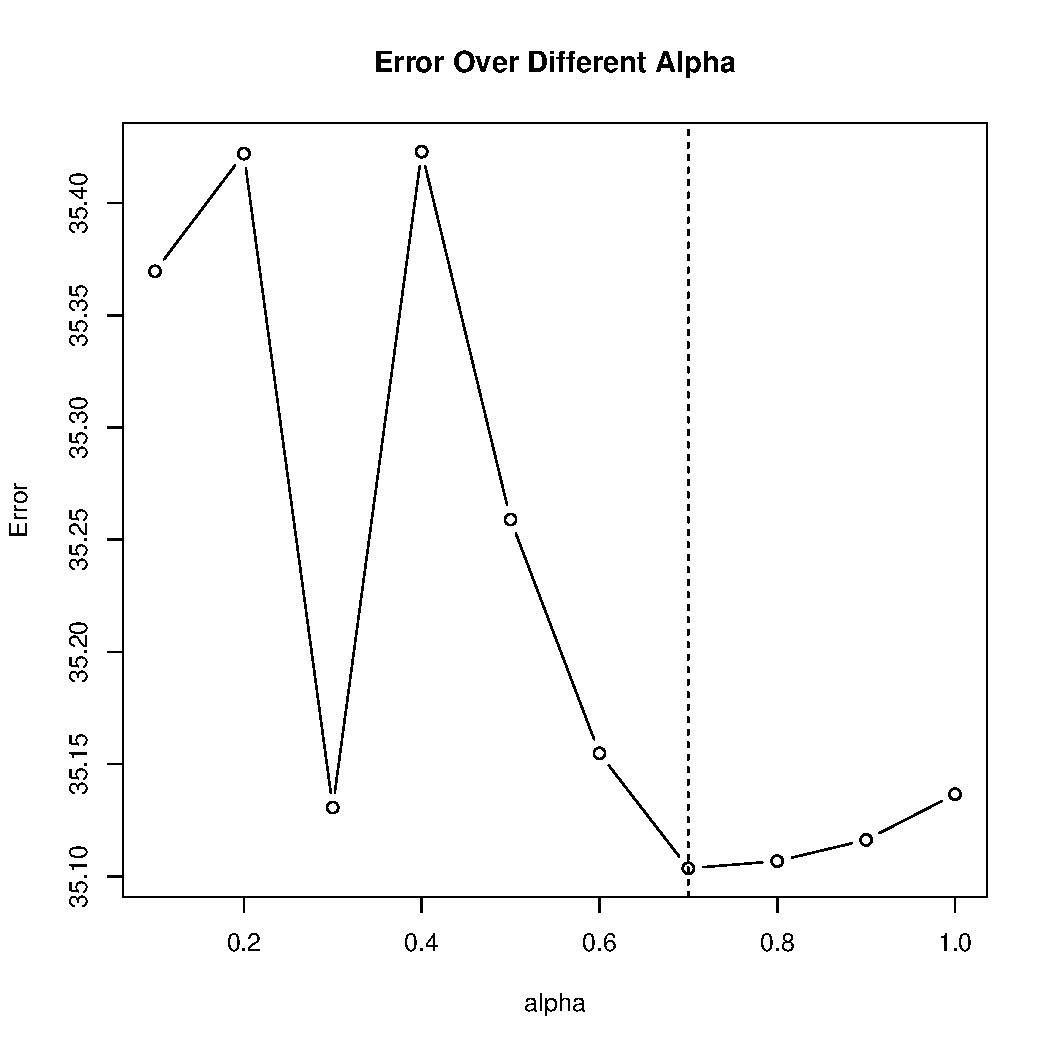
\includegraphics[width=\maxwidth]{figure/minimal-Stock1} 
\begin{kframe}\begin{alltt}
\hlcom{# So I chose alpha to be 0.7 in order to minimize the error.}
\hlstd{glmnet_fit} \hlkwb{<-} \hlkwd{glmnet}\hlstd{(price, spindex,} \hlkwc{family} \hlstd{=} \hlstr{"gaussian"}\hlstd{,} \hlkwc{standardize} \hlstd{=} \hlnum{FALSE}\hlstd{,} \hlkwc{nlambda} \hlstd{=} \hlnum{100}\hlstd{,}
    \hlkwc{alpha} \hlstd{=} \hlnum{0.7}\hlstd{)}
\hlkwd{plot}\hlstd{(glmnet_fit,} \hlkwc{xvar} \hlstd{=} \hlstr{"lambda"}\hlstd{)}
\end{alltt}
\end{kframe}
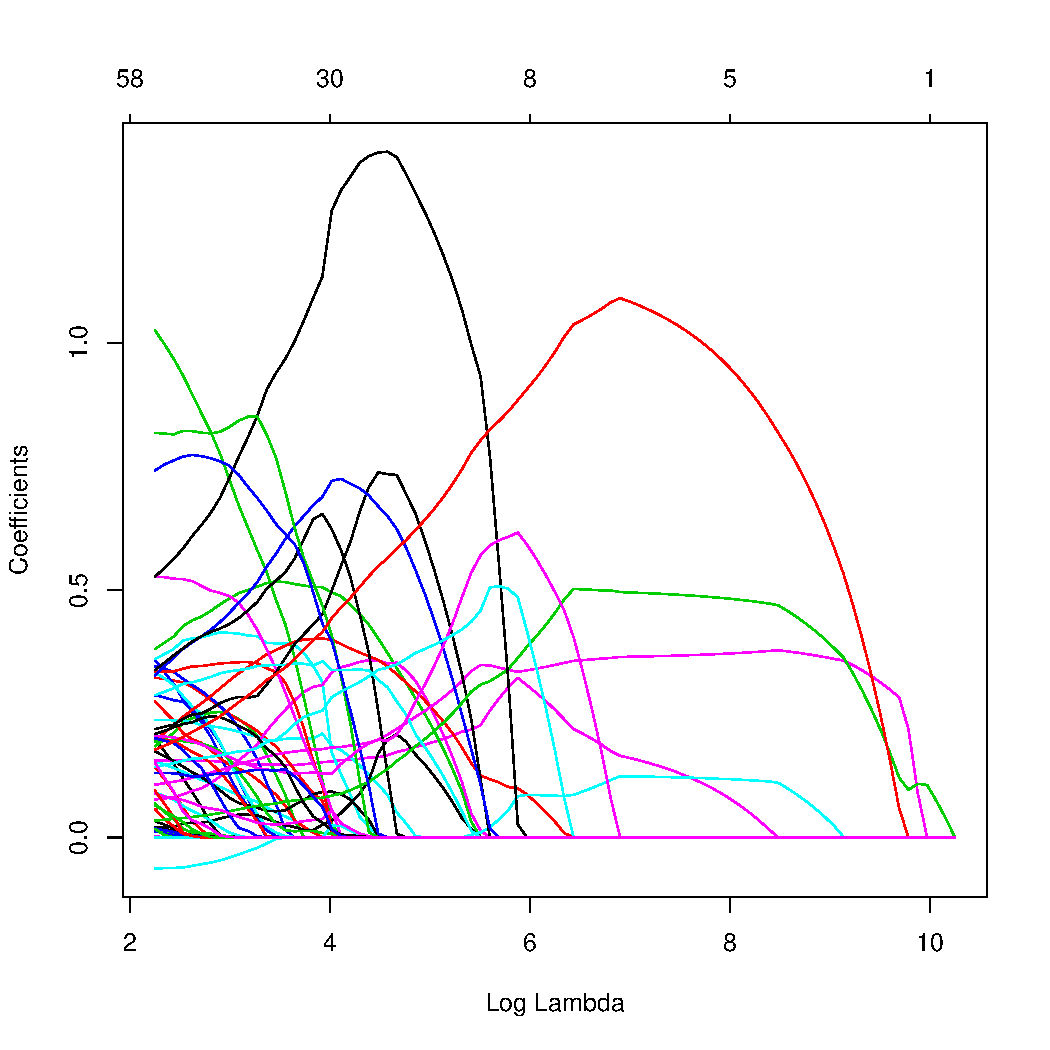
\includegraphics[width=\maxwidth]{figure/minimal-Stock2} 
\begin{kframe}\begin{alltt}
\hlstd{cv_glmnet} \hlkwb{<-} \hlkwd{cv.glmnet}\hlstd{(price, spindex,} \hlkwc{type.measure} \hlstd{=} \hlstr{"mse"}\hlstd{,} \hlkwc{family} \hlstd{=} \hlstr{"gaussian"}\hlstd{,} \hlkwc{alpha} \hlstd{=} \hlnum{0.7}\hlstd{,}
    \hlkwc{nfolds} \hlstd{=} \hlnum{10}\hlstd{)}
\hlkwd{plot}\hlstd{(cv_glmnet)}
\end{alltt}
\end{kframe}
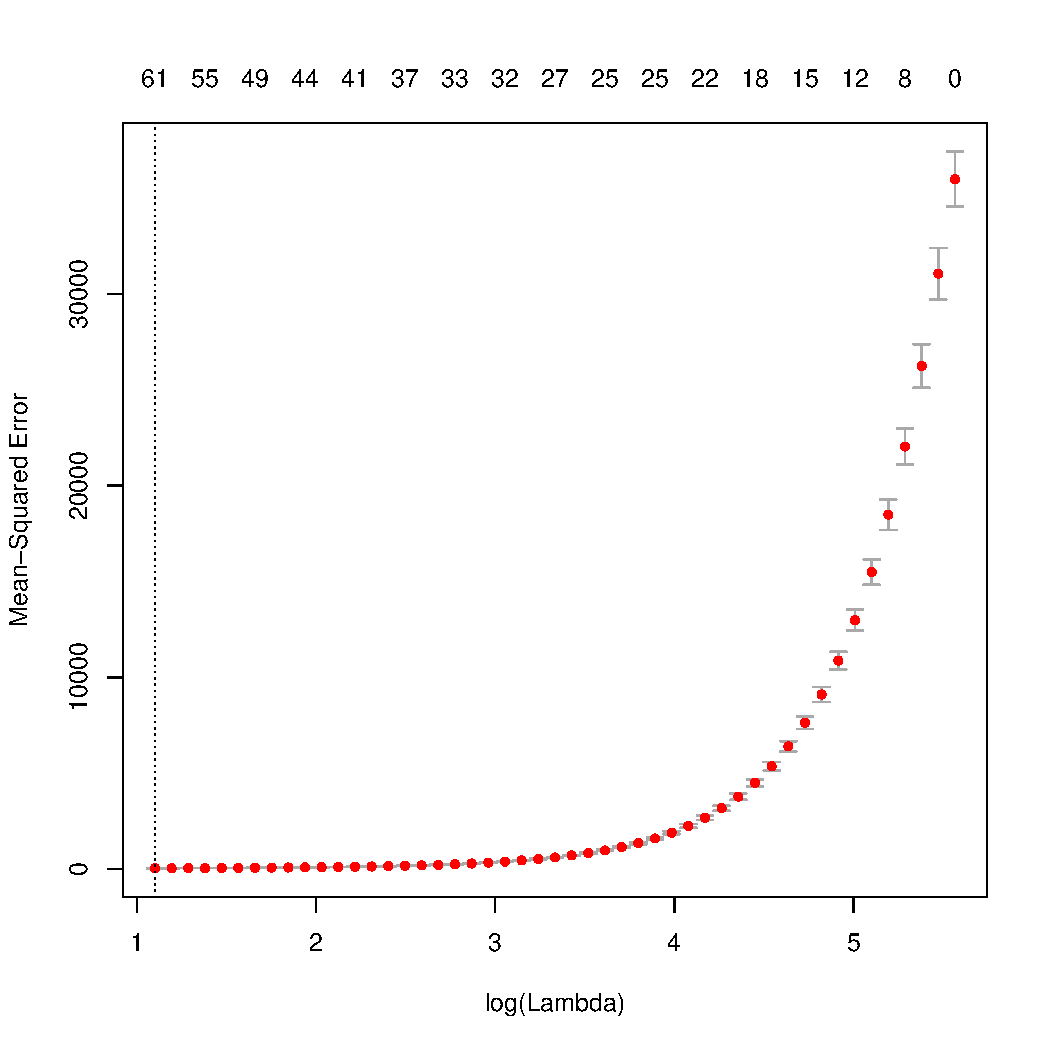
\includegraphics[width=\maxwidth]{figure/minimal-Stock3} 
\begin{kframe}\begin{alltt}
\hlstd{predict_glmnet} \hlkwb{<-} \hlkwd{predict}\hlstd{(glmnet_fit,} \hlkwc{newx} \hlstd{= price,} \hlkwc{s} \hlstd{= cv_glmnet}\hlopt{$}\hlstd{lambda.min,} \hlkwc{type} \hlstd{=} \hlstr{"link"}\hlstd{)}
\hlcom{# We need to calculate the coefficient of lasso}
\hlstd{coef_glmnet} \hlkwb{<-} \hlkwd{predict}\hlstd{(glmnet_fit,} \hlkwc{newx} \hlstd{= price,} \hlkwc{s} \hlstd{= cv_glmnet}\hlopt{$}\hlstd{lambda.min,} \hlkwc{type} \hlstd{=} \hlstr{"coefficients"}\hlstd{)}
\hlkwd{plot}\hlstd{(spindex,} \hlkwc{type} \hlstd{=} \hlstr{"p"}\hlstd{,} \hlkwc{cex} \hlstd{=} \hlnum{0.3}\hlstd{,} \hlkwc{main} \hlstd{=} \hlstr{"Best Lambda Fit"}\hlstd{)}
\hlkwd{lines}\hlstd{(predict_glmnet,} \hlkwc{col} \hlstd{=} \hlstr{"red"}\hlstd{)}
\end{alltt}
\end{kframe}
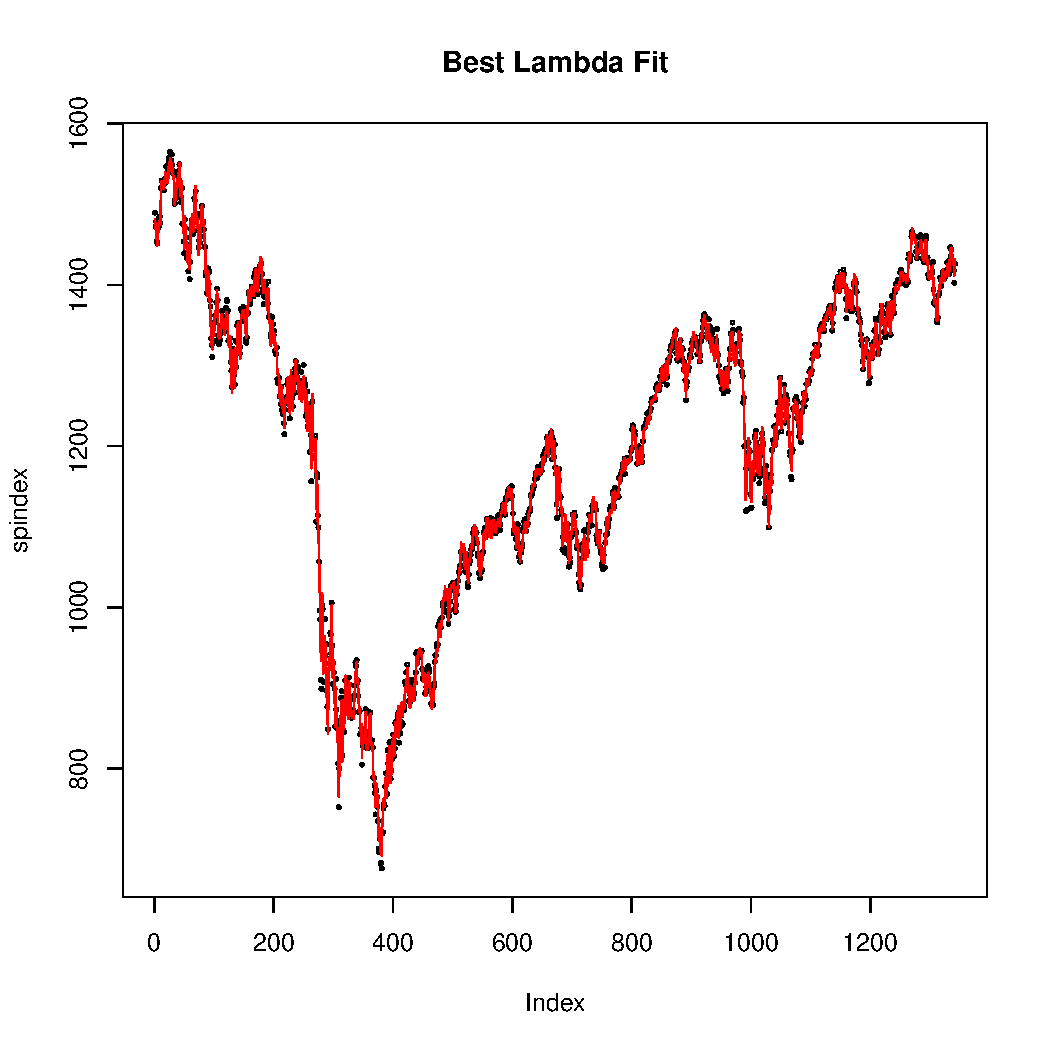
\includegraphics[width=\maxwidth]{figure/minimal-Stock4} 
\begin{kframe}\begin{alltt}
\hlcom{# The name of the company in our sparse portfolio}
\hlstd{names[}\hlkwd{which}\hlstd{(coef_glmnet} \hlopt{!=} \hlnum{0}\hlstd{)[}\hlopt{-}\hlnum{1}\hlstd{]} \hlopt{-} \hlnum{1}\hlstd{]}
\end{alltt}
\begin{verbatim}
##  [1] "3M CO"                           "ALEXION PHARMACEUTICALS INC"    
##  [3] "ALLEGHENY TECHNOLOGIES"          "ALTRIA GROUP INC"               
##  [5] "AMAZON COM INC"                  "APPLE INC"                      
##  [7] "BARD C R INC"                    "BIOGEN IDEC INC"                
##  [9] "BLACKROCK INC"                   "BOEING CO"                      
## [11] "BOSTON PROPERTIES INC"           "C F INDUSTRIES HOLDINGS INC"    
## [13] "CAPITAL ONE FINANCIAL CORP"      "CHEVRON CORP NEW"               
## [15] "CITIGROUP INC"                   "COGNIZANT TECHNOLOGY SOLS CORP" 
## [17] "CUMMINS INC"                     "DEERE & CO"                     
## [19] "DEVON ENERGY CORP NEW"           "ENTERGY CORP NEW"               
## [21] "EXXON MOBIL CORP"                "F 5 NETWORKS INC"               
## [23] "FEDEX CORP"                      "FIRST SOLAR INC"                
## [25] "FLOWSERVE CORP"                  "FLUOR CORP NEW"                 
## [27] "FRANKLIN RESOURCES INC"          "FREEPORT MCMORAN COPPER & GOLD" 
## [29] "GOLDMAN SACHS GROUP INC"         "GOOGLE INC"                     
## [31] "GRAINGER W W INC"                "HARMAN INTL INDS INC NEW"       
## [33] "HARTFORD FINANCIAL SVCS GRP INC" "INTERCONTINENTALEXCHANGE INC"   
## [35] "LOCKHEED MARTIN CORP"            "M & T BANK CORP"                
## [37] "MONSANTO CO NEW"                 "MOODYS CORP"                    
## [39] "NATIONAL OILWELL VARCO INC"      "NETFLIX INC"                    
## [41] "NORTHROP GRUMMAN CORP"           "P P G INDUSTRIES INC"           
## [43] "PACCAR INC"                      "PRICELINE COM INC"              
## [45] "PRUDENTIAL FINANCIAL INC"        "SCHLUMBERGER LTD"               
## [47] "SIMON PROPERTY GROUP INC NEW"    "STATE STREET CORP"              
## [49] "SUNTRUST BANKS INC"              "TORCHMARK CORP"                 
## [51] "UNION PACIFIC CORP"              "UNITED STATES STEEL CORP NEW"   
## [53] "VORNADO REALTY TRUST"            "WASHINGTON POST CO"             
## [55] "WELLPOINT INC"                   "WHIRLPOOL CORP"                 
## [57] "WYNN RESORTS LTD"                "ZIMMER HOLDINGS INC"
\end{verbatim}
\begin{alltt}
\hlcom{# 2)}
\hlstd{group} \hlkwb{<-} \hlkwd{seq}\hlstd{(}\hlnum{0}\hlstd{,} \hlnum{1342}\hlstd{,} \hlkwc{by} \hlstd{=} \hlnum{60}\hlstd{)}
\hlstd{portfolio} \hlkwb{<-} \hlkwa{function}\hlstd{(}\hlkwc{n}\hlstd{,} \hlkwc{folds}\hlstd{) \{}
    \hlstd{X} \hlkwb{<-} \hlstd{price[}\hlkwd{max}\hlstd{(}\hlnum{1}\hlstd{, group[n])}\hlopt{:}\hlstd{group[n} \hlopt{+} \hlnum{1}\hlstd{], ]}
    \hlstd{Y} \hlkwb{<-} \hlstd{spindex[}\hlkwd{max}\hlstd{(}\hlnum{1}\hlstd{, group[n])}\hlopt{:}\hlstd{group[n} \hlopt{+} \hlnum{1}\hlstd{]]}
    \hlstd{glmnet.fit} \hlkwb{<-} \hlkwd{glmnet}\hlstd{(X, Y,} \hlkwc{family} \hlstd{=} \hlkwd{c}\hlstd{(}\hlstr{"gaussian"}\hlstd{),} \hlkwc{standardize} \hlstd{=} \hlnum{FALSE}\hlstd{,} \hlkwc{nlambda} \hlstd{=} \hlnum{100}\hlstd{,}
        \hlkwc{alpha} \hlstd{=} \hlnum{0.7}\hlstd{)}
    \hlstd{glmnet.cv} \hlkwb{<-} \hlkwd{cv.glmnet}\hlstd{(X, Y,} \hlkwc{family} \hlstd{=} \hlstr{"gaussian"}\hlstd{,} \hlkwc{alpha} \hlstd{=} \hlnum{0.7}\hlstd{,} \hlkwc{nfolds} \hlstd{= folds)}
    \hlstd{lambda} \hlkwb{<-} \hlstd{glmnet.cv}\hlopt{$}\hlstd{lambda.min}
    \hlstd{glmnet.coef} \hlkwb{<-} \hlkwd{coef}\hlstd{(glmnet.fit,} \hlkwc{s} \hlstd{= lambda)}
    \hlstd{coefficient} \hlkwb{<-} \hlstd{glmnet.coef[}\hlkwd{which}\hlstd{(glmnet.coef} \hlopt{!=} \hlnum{0}\hlstd{)]}
    \hlstd{prediction} \hlkwb{<-} \hlkwd{predict}\hlstd{(glmnet_fit,} \hlkwc{newx} \hlstd{= X,} \hlkwc{s} \hlstd{= lambda,} \hlkwc{type} \hlstd{=} \hlstr{"link"}\hlstd{)}
    \hlkwd{return}\hlstd{(}\hlkwd{list}\hlstd{(}\hlkwc{lambda} \hlstd{= lambda,} \hlkwc{prediction} \hlstd{=} \hlkwd{as.numeric}\hlstd{(prediction),} \hlkwc{coefficient} \hlstd{= coefficient,}
        \hlkwc{compname} \hlstd{= names[}\hlkwd{which}\hlstd{(glmnet.coef} \hlopt{!=} \hlnum{0}\hlstd{)[}\hlopt{-}\hlnum{1}\hlstd{]} \hlopt{-} \hlnum{1}\hlstd{]))}
\hlstd{\}}
\hlcom{# Sample Output}
\hlkwd{portfolio}\hlstd{(}\hlnum{1}\hlstd{,} \hlnum{10}\hlstd{)}\hlopt{$}\hlstd{compname}  \hlcom{# Company List in the first 60 days.}
\end{alltt}
\begin{verbatim}
##  [1] "AVALONBAY COMMUNITIES INC"      "C M E GROUP INC"               
##  [3] "CAPITAL ONE FINANCIAL CORP"     "COGNIZANT TECHNOLOGY SOLS CORP"
##  [5] "CUMMINS INC"                    "FIRST SOLAR INC"               
##  [7] "FLUOR CORP NEW"                 "FRANKLIN RESOURCES INC"        
##  [9] "FREEPORT MCMORAN COPPER & GOLD" "GOLDMAN SACHS GROUP INC"       
## [11] "HARMAN INTL INDS INC NEW"       "NATIONAL OILWELL VARCO INC"    
## [13] "PACCAR INC"                     "SCHLUMBERGER LTD"              
## [15] "UNITED STATES STEEL CORP NEW"   "WASHINGTON POST CO"            
## [17] "WYNN RESORTS LTD"
\end{verbatim}
\begin{alltt}
\hlkwd{portfolio}\hlstd{(}\hlnum{2}\hlstd{,} \hlnum{10}\hlstd{)}\hlopt{$}\hlstd{compname}  \hlcom{# Company List in the second 60 days.}
\end{alltt}
\begin{verbatim}
## [1] "BORGWARNER INC"             "C M E GROUP INC"            "CAMERON INTERNATIONAL CORP"
## [4] "CUMMINS INC"                "FIRST SOLAR INC"            "FLUOR CORP NEW"            
## [7] "GOOGLE INC"                 "INTUITIVE SURGICAL INC"     "WASHINGTON POST CO"
\end{verbatim}
\begin{alltt}
\hlkwd{portfolio}\hlstd{(}\hlnum{3}\hlstd{,} \hlnum{10}\hlstd{)}\hlopt{$}\hlstd{compname}  \hlcom{# Company List in the third 60 days.}
\end{alltt}
\begin{verbatim}
## [1] "BLACKROCK INC"           "C M E GROUP INC"         "FIRST SOLAR INC"        
## [4] "FLUOR CORP NEW"          "GOLDMAN SACHS GROUP INC" "GOOGLE INC"             
## [7] "INTUITIVE SURGICAL INC"  "WASHINGTON POST CO"
\end{verbatim}
\begin{alltt}
\hlkwd{portfolio}\hlstd{(}\hlnum{4}\hlstd{,} \hlnum{10}\hlstd{)}\hlopt{$}\hlstd{compname}  \hlcom{# Company List in the fourth 60 days.}
\end{alltt}
\begin{verbatim}
## [1] "BLACKROCK INC"                "C M E GROUP INC"             
## [3] "FIRST SOLAR INC"              "FLUOR CORP NEW"              
## [5] "GOOGLE INC"                   "HESS CORP"                   
## [7] "INTERCONTINENTALEXCHANGE INC" "UNION PACIFIC CORP"          
## [9] "WASHINGTON POST CO"
\end{verbatim}
\begin{alltt}
\hlkwd{portfolio}\hlstd{(}\hlnum{5}\hlstd{,} \hlnum{10}\hlstd{)}\hlopt{$}\hlstd{compname}  \hlcom{# Company List in the fifth 60 days.}
\end{alltt}
\begin{verbatim}
## [1] "FIRST SOLAR INC"         "GOLDMAN SACHS GROUP INC" "GOOGLE INC"             
## [4] "INTUITIVE SURGICAL INC"  "WASHINGTON POST CO"
\end{verbatim}
\begin{alltt}
\hlkwd{portfolio}\hlstd{(}\hlnum{10}\hlstd{,} \hlnum{10}\hlstd{)}\hlopt{$}\hlstd{compname}  \hlcom{# Company List in the tenth 60 days.}
\end{alltt}
\begin{verbatim}
##  [1] "APPLE INC"                      "BLACKROCK INC"                 
##  [3] "C M E GROUP INC"                "EBIX INC"                      
##  [5] "FLOWSERVE CORP"                 "FREEPORT MCMORAN COPPER & GOLD"
##  [7] "INTUITIVE SURGICAL INC"         "MASTERCARD INC"                
##  [9] "PRICELINE COM INC"              "WYNN RESORTS LTD"
\end{verbatim}
\begin{alltt}
\hlkwd{portfolio}\hlstd{(}\hlnum{15}\hlstd{,} \hlnum{10}\hlstd{)}\hlopt{$}\hlstd{compname}  \hlcom{# Company List in the fiftith 60 days.}
\end{alltt}
\begin{verbatim}
##  [1] "APPLE INC"                      "AUTOZONE INC"                  
##  [3] "BALL CORP"                      "C M E GROUP INC"               
##  [5] "FLOWSERVE CORP"                 "FREEPORT MCMORAN COPPER & GOLD"
##  [7] "GOLDMAN SACHS GROUP INC"        "GOOGLE INC"                    
##  [9] "INTUITIVE SURGICAL INC"         "LAUDER ESTEE COS INC"          
## [11] "NETFLIX INC"                    "PRICELINE COM INC"             
## [13] "SCHLUMBERGER LTD"               "WASHINGTON POST CO"
\end{verbatim}
\begin{alltt}
\hlstd{CME} \hlkwb{<-} \hlkwd{matrix}\hlstd{(}\hlnum{0}\hlstd{,} \hlnum{22}\hlstd{)}
\hlkwa{for} \hlstd{(i} \hlkwa{in} \hlnum{1}\hlopt{:}\hlnum{22}\hlstd{) \{}
    \hlkwa{if} \hlstd{(}\hlkwd{sum}\hlstd{(}\hlkwd{portfolio}\hlstd{(i,} \hlnum{10}\hlstd{)}\hlopt{$}\hlstd{compname} \hlopt{==} \hlstr{"C M E GROUP INC"}\hlstd{)} \hlopt{!=} \hlnum{0}\hlstd{) \{}
        \hlstd{j} \hlkwb{<-} \hlkwd{which}\hlstd{(}\hlkwd{portfolio}\hlstd{(i,} \hlnum{10}\hlstd{)}\hlopt{$}\hlstd{compname} \hlopt{==} \hlstr{"C M E GROUP INC"}\hlstd{)}
        \hlstd{CME[i]} \hlkwb{<-} \hlkwd{portfolio}\hlstd{(i,} \hlnum{10}\hlstd{)}\hlopt{$}\hlstd{coefficient[(j} \hlopt{+} \hlnum{1}\hlstd{)]}
    \hlstd{\}}
\hlstd{\}}
\hlkwd{plot}\hlstd{(CME,} \hlkwc{main} \hlstd{=} \hlstr{"CME weights in replicating S&P500 index"}\hlstd{,} \hlkwc{type} \hlstd{=} \hlstr{"b"}\hlstd{,} \hlkwc{xlab} \hlstd{=} \hlstr{"Different portfolios"}\hlstd{)}
\end{alltt}
\end{kframe}
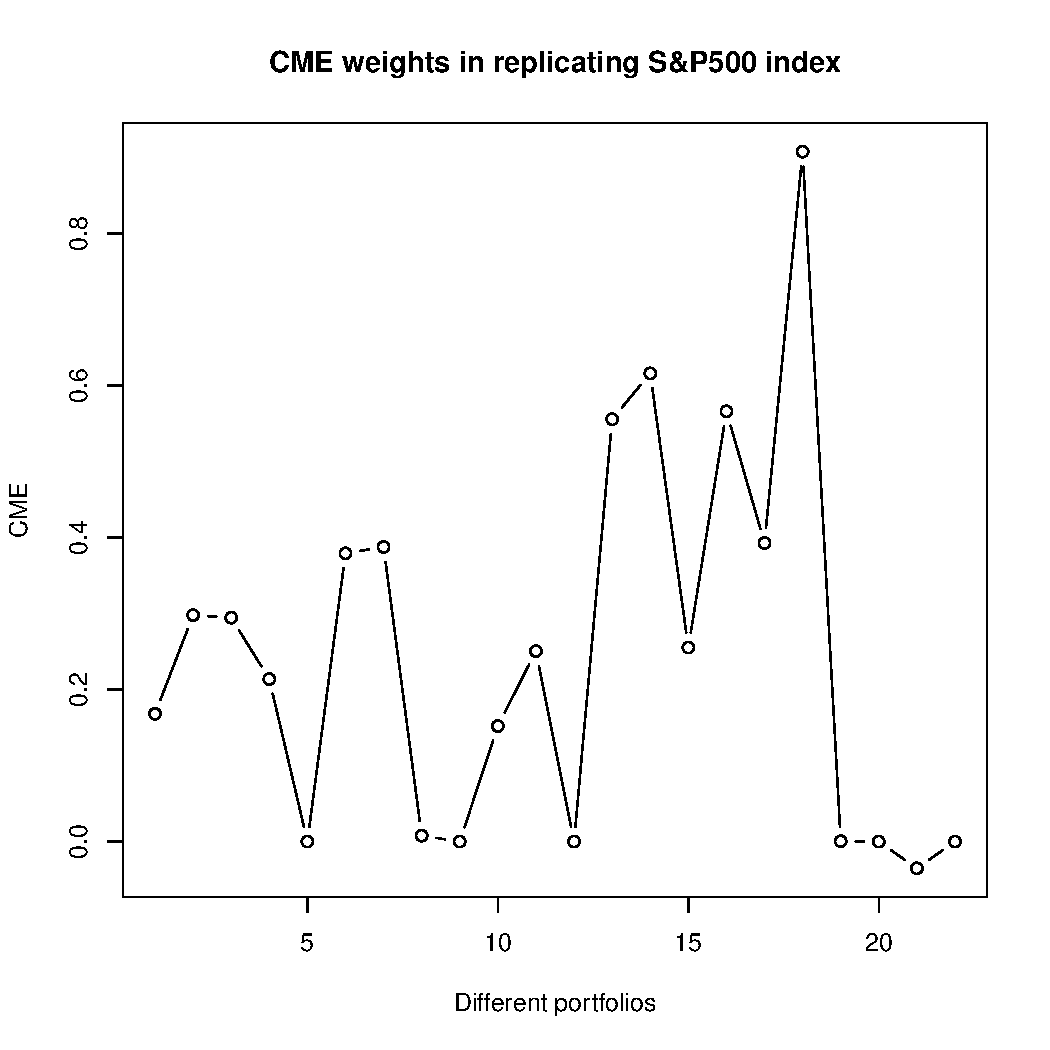
\includegraphics[width=\maxwidth]{figure/minimal-Stock5} 
\begin{kframe}\begin{alltt}
\hlcom{# I need to figure out the stability of company list.}
\hlstd{number_comp} \hlkwb{<-} \hlkwd{matrix}\hlstd{(}\hlnum{NA}\hlstd{,} \hlnum{22}\hlstd{)}
\hlstd{name_comp} \hlkwb{<-} \hlkwd{matrix}\hlstd{(}\hlnum{NA}\hlstd{,} \hlnum{22}\hlstd{,} \hlnum{17}\hlstd{)}
\hlkwa{for} \hlstd{(i} \hlkwa{in} \hlnum{1}\hlopt{:}\hlnum{22}\hlstd{) \{}
    \hlstd{number_comp[i, ]} \hlkwb{<-} \hlkwd{length}\hlstd{(}\hlkwd{portfolio}\hlstd{(i,} \hlnum{10}\hlstd{)}\hlopt{$}\hlstd{compname)}
\hlstd{\}}
\hlkwd{plot}\hlstd{(number_comp,} \hlkwc{main} \hlstd{=} \hlstr{"Number of Companies in Portfolio & SP500 Index"}\hlstd{,} \hlkwc{type} \hlstd{=} \hlstr{"b"}\hlstd{,} \hlkwc{xlab} \hlstd{=} \hlstr{"Portfolios Every 60 Days"}\hlstd{)}
\end{alltt}
\end{kframe}
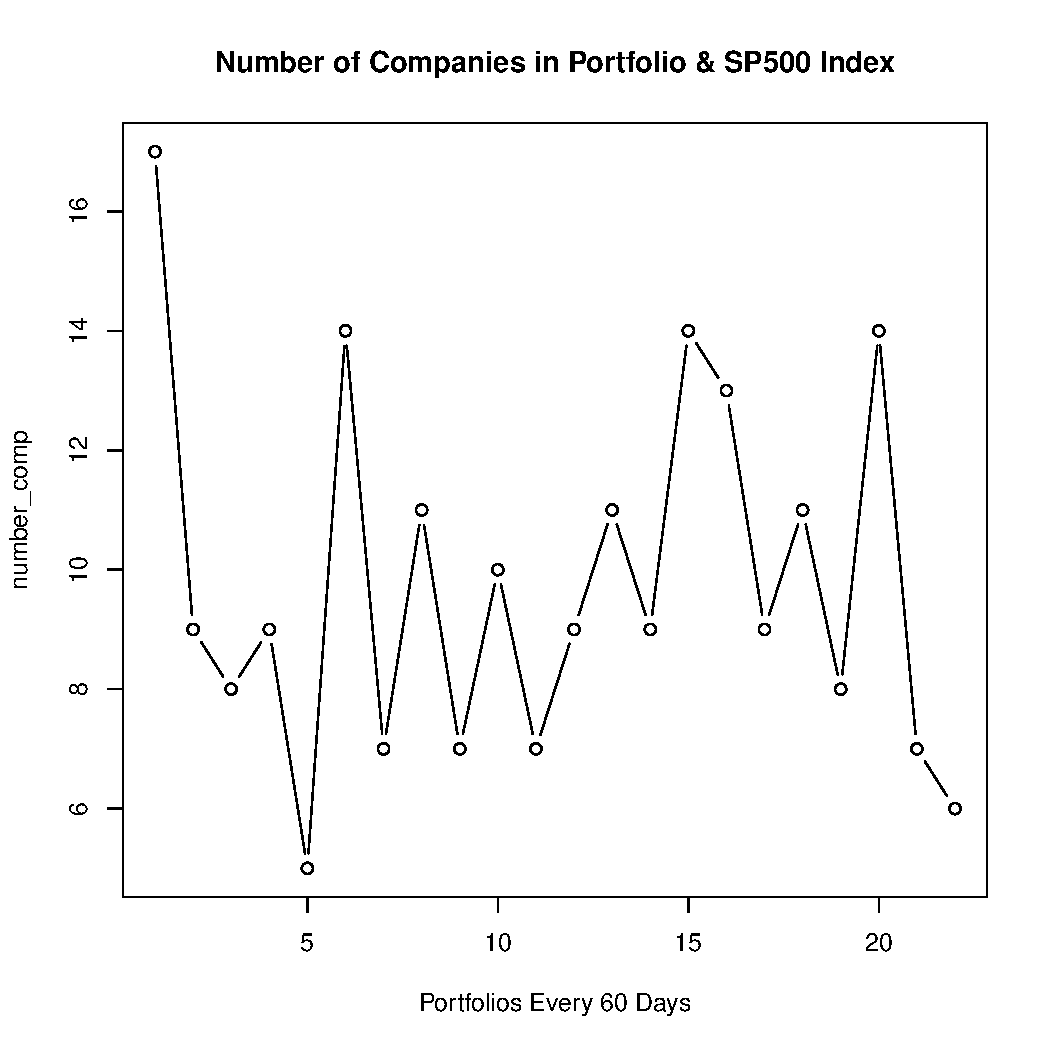
\includegraphics[width=\maxwidth]{figure/minimal-Stock6} 
\begin{kframe}\begin{alltt}
\hlcom{# 4).}
\hlstd{Return.lasso} \hlkwb{<-} \hlkwd{glmnet}\hlstd{(price, SPReturn,} \hlkwc{family} \hlstd{=} \hlstr{"gaussian"}\hlstd{,} \hlkwc{standardize} \hlstd{=} \hlnum{FALSE}\hlstd{,} \hlkwc{alpha} \hlstd{=} \hlnum{1}\hlstd{)}
\hlstd{Return.cv} \hlkwb{<-} \hlkwd{cv.glmnet}\hlstd{(price,} \hlkwd{as.matrix}\hlstd{(SPReturn),} \hlkwc{family} \hlstd{=} \hlstr{"gaussian"}\hlstd{,} \hlkwc{alpha} \hlstd{=} \hlnum{1}\hlstd{)}
\hlkwd{plot}\hlstd{(Return.cv,} \hlkwc{main} \hlstd{=} \hlstr{"Cross Validation For Sparse Porfolio of Returns"}\hlstd{)}
\end{alltt}
\end{kframe}
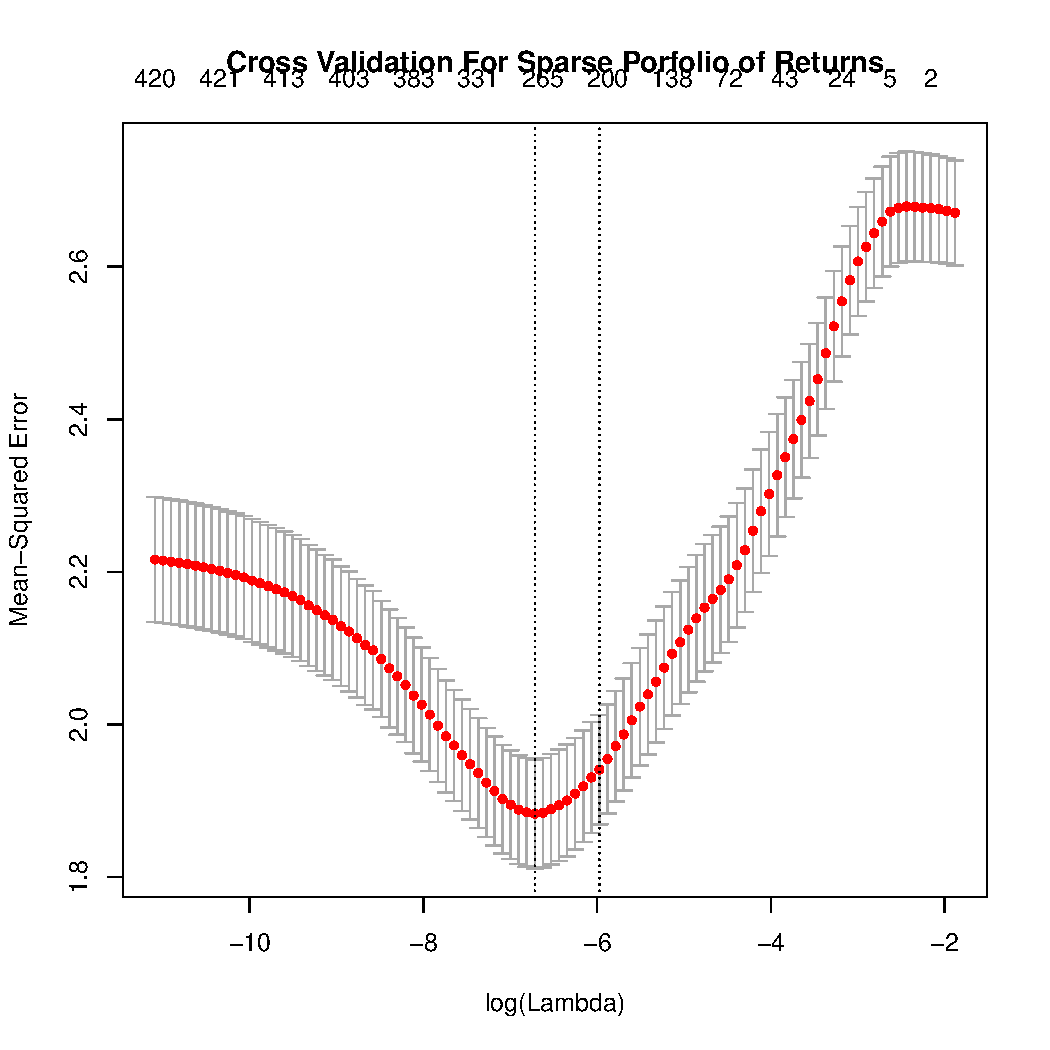
\includegraphics[width=\maxwidth]{figure/minimal-Stock7} 
\begin{kframe}\begin{alltt}
\hlstd{Return.coef} \hlkwb{<-} \hlkwd{coef}\hlstd{(Return.lasso,} \hlkwc{s} \hlstd{= Return.cv}\hlopt{$}\hlstd{lambda.min,} \hlkwc{alpha} \hlstd{=} \hlnum{1}\hlstd{)}
\hlkwd{length}\hlstd{(}\hlkwd{which}\hlstd{(Return.coef} \hlopt{!=} \hlnum{0}\hlstd{))} \hlopt{-} \hlnum{1}  \hlcom{# The number of coefficients minus one intercept}
\end{alltt}
\begin{verbatim}
## [1] 408
\end{verbatim}
\begin{alltt}
\hlstd{portfolio_return} \hlkwb{<-} \hlkwa{function}\hlstd{(}\hlkwc{n}\hlstd{,} \hlkwc{folds}\hlstd{) \{}
    \hlstd{X} \hlkwb{<-} \hlstd{price[}\hlkwd{max}\hlstd{(}\hlnum{1}\hlstd{, group[n])}\hlopt{:}\hlstd{group[n} \hlopt{+} \hlnum{1}\hlstd{], ]}
    \hlstd{Y} \hlkwb{<-} \hlstd{SPReturn[}\hlkwd{max}\hlstd{(}\hlnum{1}\hlstd{, group[n])}\hlopt{:}\hlstd{group[n} \hlopt{+} \hlnum{1}\hlstd{]]}
    \hlstd{glmnet.fit} \hlkwb{<-} \hlkwd{glmnet}\hlstd{(X, Y,} \hlkwc{family} \hlstd{=} \hlkwd{c}\hlstd{(}\hlstr{"gaussian"}\hlstd{),} \hlkwc{standardize} \hlstd{=} \hlnum{FALSE}\hlstd{,} \hlkwc{nlambda} \hlstd{=} \hlnum{100}\hlstd{,}
        \hlkwc{alpha} \hlstd{=} \hlnum{0.7}\hlstd{)}
    \hlstd{glmnet.cv} \hlkwb{<-} \hlkwd{cv.glmnet}\hlstd{(X, Y,} \hlkwc{family} \hlstd{=} \hlstr{"gaussian"}\hlstd{,} \hlkwc{alpha} \hlstd{=} \hlnum{0.7}\hlstd{,} \hlkwc{nfolds} \hlstd{= folds)}
    \hlstd{lambda} \hlkwb{<-} \hlstd{glmnet.cv}\hlopt{$}\hlstd{lambda.min}
    \hlstd{glmnet.coef} \hlkwb{<-} \hlkwd{coef}\hlstd{(glmnet.fit,} \hlkwc{s} \hlstd{= lambda)}
    \hlstd{coefficient} \hlkwb{<-} \hlstd{glmnet.coef[}\hlkwd{which}\hlstd{(glmnet.coef} \hlopt{!=} \hlnum{0}\hlstd{)]}
    \hlstd{prediction} \hlkwb{<-} \hlkwd{predict}\hlstd{(glmnet_fit,} \hlkwc{newx} \hlstd{= X,} \hlkwc{s} \hlstd{= lambda,} \hlkwc{type} \hlstd{=} \hlstr{"link"}\hlstd{)}
    \hlkwd{return}\hlstd{(}\hlkwd{list}\hlstd{(}\hlkwc{lambda} \hlstd{= lambda,} \hlkwc{prediction} \hlstd{=} \hlkwd{as.numeric}\hlstd{(prediction),} \hlkwc{coefficient} \hlstd{= coefficient,}
        \hlkwc{compname} \hlstd{= names[}\hlkwd{which}\hlstd{(glmnet.coef} \hlopt{!=} \hlnum{0}\hlstd{)[}\hlopt{-}\hlnum{1}\hlstd{]} \hlopt{-} \hlnum{1}\hlstd{]))}
\hlstd{\}}
\hlkwd{portfolio_return}\hlstd{(}\hlnum{1}\hlstd{,} \hlnum{10}\hlstd{)}\hlopt{$}\hlstd{compname}
\end{alltt}
\begin{verbatim}
##  [1] "A F L A C INC"                    "AMAZON COM INC"                  
##  [3] "APOLLO GROUP INC"                 "APPLE INC"                       
##  [5] "ASSURANT INC"                     "AVALONBAY COMMUNITIES INC"       
##  [7] "BIOGEN IDEC INC"                  "CELGENE CORP"                    
##  [9] "CONSOL ENERGY INC"                "DOMINION RESOURCES INC VA NEW"   
## [11] "F M C CORP"                       "FEDEX CORP"                      
## [13] "FIRST SOLAR INC"                  "FLIR SYSTEMS INC"                
## [15] "FLOWSERVE CORP"                   "FRANKLIN RESOURCES INC"          
## [17] "FREEPORT MCMORAN COPPER & GOLD"   "GARMIN LTD"                      
## [19] "GOOGLE INC"                       "HARTFORD FINANCIAL SVCS GRP INC" 
## [21] "HUMANA INC"                       "INTERCONTINENTALEXCHANGE INC"    
## [23] "INTERNATIONAL BUSINESS MACHS COR" "INTUITIVE SURGICAL INC"          
## [25] "JACOBS ENGINEERING GROUP INC"     "KIMBERLY CLARK CORP"             
## [27] "L 3 COMMUNICATIONS HLDGS INC"     "LEGG MASON INC"                  
## [29] "M & T BANK CORP"                  "P N C FINANCIAL SERVICES GRP INC"
## [31] "PACCAR INC"                       "PARKER HANNIFIN CORP"            
## [33] "STATE STREET CORP"                "T ROWE PRICE GROUP INC"          
## [35] "UNION PACIFIC CORP"
\end{verbatim}
\begin{alltt}
\hlkwd{portfolio_return}\hlstd{(}\hlnum{2}\hlstd{,} \hlnum{10}\hlstd{)}\hlopt{$}\hlstd{compname}
\end{alltt}
\begin{verbatim}
##  [1] "ABERCROMBIE & FITCH CO"           "ALLEGHENY TECHNOLOGIES"          
##  [3] "AMERICAN EXPRESS CO"              "APACHE CORP"                     
##  [5] "APOLLO GROUP INC"                 "BAKER HUGHES INC"                
##  [7] "BLACKROCK INC"                    "C M E GROUP INC"                 
##  [9] "CAMERON INTERNATIONAL CORP"       "CELGENE CORP"                    
## [11] "CERNER CORP"                      "CUMMINS INC"                     
## [13] "DEERE & CO"                       "DENBURY RESOURCES INC"           
## [15] "ENTERGY CORP NEW"                 "EOG RESOURCES INC"               
## [17] "FIRST SOLAR INC"                  "FREEPORT MCMORAN COPPER & GOLD"  
## [19] "GAMESTOP CORP NEW"                "GOOGLE INC"                      
## [21] "HARMAN INTL INDS INC NEW"         "INTERCONTINENTALEXCHANGE INC"    
## [23] "INTERNATIONAL BUSINESS MACHS COR" "INTUITIVE SURGICAL INC"          
## [25] "JACOBS ENGINEERING GROUP INC"     "LABORATORY CORP AMERICA HLDGS"   
## [27] "LAM RESH CORP"                    "LEGG MASON INC"                  
## [29] "M & T BANK CORP"                  "MASTERCARD INC"                  
## [31] "MONSANTO CO NEW"                  "NORDSTROM INC"                   
## [33] "NORTHROP GRUMMAN CORP"            "P P G INDUSTRIES INC"            
## [35] "PACCAR INC"                       "PEPSICO INC"                     
## [37] "PRICELINE COM INC"                "PRINCIPAL FINANCIAL GROUP INC"   
## [39] "PUBLIC SERVICE ENTERPRISE GP INC" "SHERWIN WILLIAMS CO"             
## [41] "TARGET CORP"                      "TEXTRON INC"                     
## [43] "UNITED STATES STEEL CORP NEW"     "V F CORP"                        
## [45] "WASHINGTON POST CO"               "WYNN RESORTS LTD"
\end{verbatim}
\begin{alltt}
\hlkwd{portfolio_return}\hlstd{(}\hlnum{5}\hlstd{,} \hlnum{10}\hlstd{)}\hlopt{$}\hlstd{compname}
\end{alltt}
\begin{verbatim}
##  [1] "ALEXION PHARMACEUTICALS INC"     "APACHE CORP"                    
##  [3] "APPLE INC"                       "AVALONBAY COMMUNITIES INC"      
##  [5] "BLACKROCK INC"                   "BOSTON PROPERTIES INC"          
##  [7] "C F INDUSTRIES HOLDINGS INC"     "C M E GROUP INC"                
##  [9] "CHUBB CORP"                      "CONSOL ENERGY INC"              
## [11] "DIAMOND OFFSHORE DRILLING INC"   "DUN & BRADSTREET CORP DEL NEW"  
## [13] "EXXON MOBIL CORP"                "FIRST SOLAR INC"                
## [15] "FRANKLIN RESOURCES INC"          "GOLDMAN SACHS GROUP INC"        
## [17] "GOOGLE INC"                      "HARTFORD FINANCIAL SVCS GRP INC"
## [19] "INTERCONTINENTALEXCHANGE INC"    "INTUITIVE SURGICAL INC"         
## [21] "JOHNSON & JOHNSON"               "L 3 COMMUNICATIONS HLDGS INC"   
## [23] "M & T BANK CORP"                 "METLIFE INC"                    
## [25] "NIKE INC"                        "NORTHERN TRUST CORP"            
## [27] "SIMON PROPERTY GROUP INC NEW"    "TORCHMARK CORP"                 
## [29] "V F CORP"                        "VORNADO REALTY TRUST"           
## [31] "WASHINGTON POST CO"              "WYNN RESORTS LTD"
\end{verbatim}
\begin{alltt}
\hlkwd{portfolio_return}\hlstd{(}\hlnum{10}\hlstd{,} \hlnum{10}\hlstd{)}\hlopt{$}\hlstd{compname}
\end{alltt}
\begin{verbatim}
##  [1] "ANADARKO PETROLEUM CORP"          "APOLLO GROUP INC"                
##  [3] "AUTOZONE INC"                     "BARD C R INC"                    
##  [5] "BAXTER INTERNATIONAL INC"         "BEST BUY COMPANY INC"            
##  [7] "BLACKROCK INC"                    "C S X CORP"                      
##  [9] "CABOT OIL & GAS CORP"             "CONSOL ENERGY INC"               
## [11] "CUMMINS INC"                      "DEERE & CO"                      
## [13] "DIAMOND OFFSHORE DRILLING INC"    "EASTMAN CHEMICAL CO"             
## [15] "EBIX INC"                         "ENTERGY CORP NEW"                
## [17] "EXXON MOBIL CORP"                 "GARMIN LTD"                      
## [19] "GOLDMAN SACHS GROUP INC"          "GOOGLE INC"                      
## [21] "HEALTH CARE REIT INC"             "INTERCONTINENTALEXCHANGE INC"    
## [23] "INTUITIVE SURGICAL INC"           "JOY GLOBAL INC"                  
## [25] "KIMBERLY CLARK CORP"              "LEGG MASON INC"                  
## [27] "M & T BANK CORP"                  "MASTERCARD INC"                  
## [29] "MONSANTO CO NEW"                  "NORTHERN TRUST CORP"             
## [31] "PRICELINE COM INC"                "REGENERON PHARMACEUTICALS INC"   
## [33] "SEMPRA ENERGY"                    "SIGMA ALDRICH CORP"              
## [35] "SMUCKER J M CO"                   "STARWOOD HOTELS & REST WLDWD INC"
## [37] "STERICYCLE INC"                   "V F CORP"                        
## [39] "VARIAN MEDICAL SYSTEMS INC"       "VORNADO REALTY TRUST"            
## [41] "WYNN RESORTS LTD"
\end{verbatim}
\begin{alltt}
\hlkwd{portfolio_return}\hlstd{(}\hlnum{15}\hlstd{,} \hlnum{10}\hlstd{)}\hlopt{$}\hlstd{compname}
\end{alltt}
\begin{verbatim}
##  [1] "AGILENT TECHNOLOGIES INC"         "ALEXION PHARMACEUTICALS INC"     
##  [3] "APACHE CORP"                      "APOLLO GROUP INC"                
##  [5] "APPLE INC"                        "AUTOZONE INC"                    
##  [7] "AVALONBAY COMMUNITIES INC"        "BALL CORP"                       
##  [9] "C M E GROUP INC"                  "CH ROBINSON WORLDWIDE INC"       
## [11] "CONSOL ENERGY INC"                "F 5 NETWORKS INC"                
## [13] "F M C TECHNOLOGIES INC"           "FIRST SOLAR INC"                 
## [15] "FLOWSERVE CORP"                   "FREEPORT MCMORAN COPPER & GOLD"  
## [17] "GOLDMAN SACHS GROUP INC"          "GOOGLE INC"                      
## [19] "GRAINGER W W INC"                 "HELMERICH & PAYNE INC"           
## [21] "INTERNATIONAL BUSINESS MACHS COR" "INTUITIVE SURGICAL INC"          
## [23] "JOY GLOBAL INC"                   "LABORATORY CORP AMERICA HLDGS"   
## [25] "LOCKHEED MARTIN CORP"             "M & T BANK CORP"                 
## [27] "MASTERCARD INC"                   "MONSANTO CO NEW"                 
## [29] "NATIONAL OILWELL VARCO INC"       "NETFLIX INC"                     
## [31] "NEWMONT MINING CORP"              "NORFOLK SOUTHERN CORP"           
## [33] "P N C FINANCIAL SERVICES GRP INC" "PALL CORP"                       
## [35] "PRICELINE COM INC"                "ROCKWELL AUTOMATION INC"         
## [37] "ROSS STORES INC"                  "STARWOOD HOTELS & REST WLDWD INC"
## [39] "UNITED STATES STEEL CORP NEW"     "WASHINGTON POST CO"              
## [41] "WESTERN DIGITAL CORP"             "WISCONSIN ENERGY CORP"           
## [43] "WYNN RESORTS LTD"
\end{verbatim}
\begin{alltt}
\hlkwd{portfolio_return}\hlstd{(}\hlnum{20}\hlstd{,} \hlnum{10}\hlstd{)}\hlopt{$}\hlstd{compname}
\end{alltt}
\begin{verbatim}
##  [1] "ABERCROMBIE & FITCH CO"          "AKAMAI TECHNOLOGIES INC"        
##  [3] "ALEXION PHARMACEUTICALS INC"     "AMAZON COM INC"                 
##  [5] "APPLE INC"                       "AVALONBAY COMMUNITIES INC"      
##  [7] "BAXTER INTERNATIONAL INC"        "BIOGEN IDEC INC"                
##  [9] "C M E GROUP INC"                 "CELGENE CORP"                   
## [11] "CROWN CASTLE INTERNATIONAL CORP" "EDWARDS LIFESCIENCES CORP"      
## [13] "F 5 NETWORKS INC"                "FLOWSERVE CORP"                 
## [15] "FOSSIL INC"                      "GOLDMAN SACHS GROUP INC"        
## [17] "GOOGLE INC"                      "INTERCONTINENTALEXCHANGE INC"   
## [19] "INTUITIVE SURGICAL INC"          "JOY GLOBAL INC"                 
## [21] "KOHLS CORP"                      "M & T BANK CORP"                
## [23] "MASTERCARD INC"                  "NOBLE ENERGY INC"               
## [25] "ONEOK INC NEW"                   "P P G INDUSTRIES INC"           
## [27] "PRECISION CASTPARTS CORP"        "PRICELINE COM INC"              
## [29] "SALESFORCE COM INC"              "SANDISK CORP"                   
## [31] "SCHLUMBERGER LTD"                "UNITED STATES STEEL CORP NEW"   
## [33] "WASHINGTON POST CO"
\end{verbatim}
\begin{alltt}
\hlstd{number_comp_return} \hlkwb{<-} \hlkwd{matrix}\hlstd{(}\hlnum{NA}\hlstd{,} \hlnum{22}\hlstd{)}
\hlkwa{for} \hlstd{(i} \hlkwa{in} \hlnum{1}\hlopt{:}\hlnum{22}\hlstd{) \{}
    \hlstd{number_comp_return[i, ]} \hlkwb{<-} \hlkwd{length}\hlstd{(}\hlkwd{portfolio_return}\hlstd{(i,} \hlnum{10}\hlstd{)}\hlopt{$}\hlstd{compname)}
\hlstd{\}}
\hlkwd{plot}\hlstd{(number_comp_return,} \hlkwc{main} \hlstd{=} \hlstr{"Number of Companies in Portfolio & SP500 Return"}\hlstd{,} \hlkwc{type} \hlstd{=} \hlstr{"b"}\hlstd{,}
    \hlkwc{xlab} \hlstd{=} \hlstr{"Portfolios Every 60 Days"}\hlstd{)}
\end{alltt}
\end{kframe}
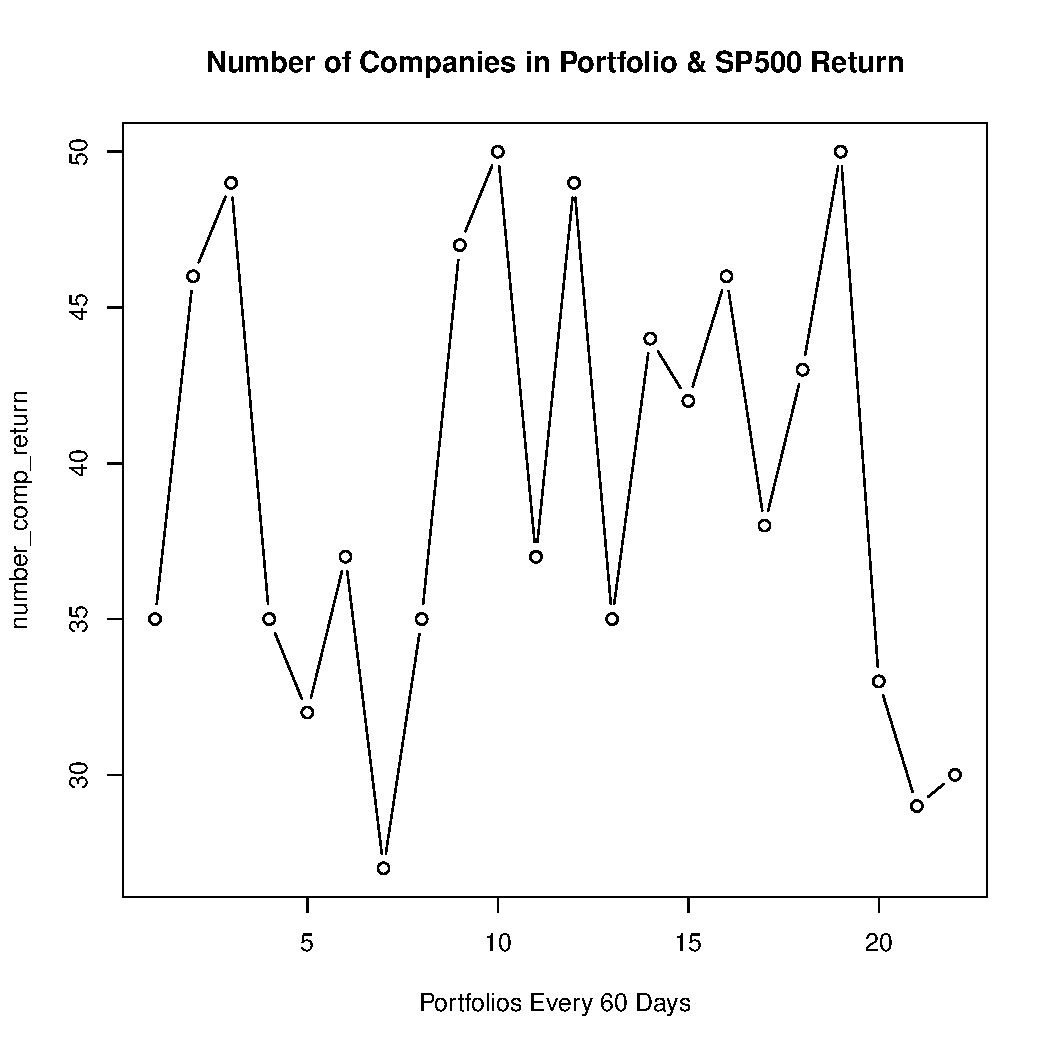
\includegraphics[width=\maxwidth]{figure/minimal-Stock8} 
\begin{kframe}\begin{alltt}
\hlcom{# 5).}
\hlstd{sp500_lm} \hlkwb{<-} \hlkwd{lm}\hlstd{(spindex[}\hlnum{1}\hlopt{:}\hlnum{800}\hlstd{]} \hlopt{~} \hlstd{price[}\hlnum{1}\hlopt{:}\hlnum{800}\hlstd{, ])}
\hlstd{prediction} \hlkwb{<-} \hlkwd{predict}\hlstd{(sp500_lm,} \hlkwc{interval} \hlstd{=} \hlstr{"none"}\hlstd{,} \hlkwc{type} \hlstd{=} \hlstr{"response"}\hlstd{)}
\hlkwd{sum}\hlstd{((prediction} \hlopt{-} \hlstd{spindex[}\hlnum{1}\hlopt{:}\hlnum{800}\hlstd{])}\hlopt{^}\hlnum{2}\hlstd{)}\hlopt{/}\hlnum{800}
\end{alltt}
\begin{verbatim}
## [1] 0.09587
\end{verbatim}
\begin{alltt}
\hlstd{lm.test} \hlkwb{<-} \hlkwd{cbind}\hlstd{(}\hlkwd{rep}\hlstd{(}\hlnum{1}\hlstd{,} \hlnum{542}\hlstd{), price[}\hlnum{801}\hlopt{:}\hlnum{1342}\hlstd{, ])} \hlopt \hlstd{sp500_lm}\hlopt{$}\hlstd{coefficients}
\hlkwd{sum}\hlstd{((lm.test} \hlopt{-} \hlstd{spindex[}\hlnum{801}\hlopt{:}\hlnum{1342}\hlstd{])}\hlopt{^}\hlnum{2}\hlstd{)}\hlopt{/}\hlnum{542}
\end{alltt}
\begin{verbatim}
## [1] 275
\end{verbatim}
\begin{alltt}
\hlstd{sp500_ridge} \hlkwb{<-} \hlkwd{glmnet}\hlstd{(price[}\hlnum{1}\hlopt{:}\hlnum{800}\hlstd{, ], spindex[}\hlnum{1}\hlopt{:}\hlnum{800}\hlstd{],} \hlkwc{standardize} \hlstd{=} \hlnum{FALSE}\hlstd{,} \hlkwc{family} \hlstd{=} \hlstr{"gaussian"}\hlstd{,}
    \hlkwc{alpha} \hlstd{=} \hlnum{1}\hlstd{)}
\hlstd{ridge.cv} \hlkwb{<-} \hlkwd{cv.glmnet}\hlstd{(price[}\hlnum{1}\hlopt{:}\hlnum{800}\hlstd{, ], spindex[}\hlnum{1}\hlopt{:}\hlnum{800}\hlstd{],} \hlkwc{family} \hlstd{=} \hlstr{"gaussian"}\hlstd{,} \hlkwc{type.measure} \hlstd{=} \hlstr{"mse"}\hlstd{,}
    \hlkwc{alpha} \hlstd{=} \hlnum{1}\hlstd{)}
\hlstd{ridge.fit} \hlkwb{<-} \hlkwd{predict}\hlstd{(ridge.cv, price[}\hlnum{801}\hlopt{:}\hlnum{1342}\hlstd{, ],} \hlkwc{s} \hlstd{= ridge.cv}\hlopt{$}\hlstd{lambda.min,} \hlkwc{type} \hlstd{=} \hlstr{"link"}\hlstd{)}
\hlkwd{sum}\hlstd{((ridge.fit} \hlopt{-} \hlstd{spindex[}\hlnum{801}\hlopt{:}\hlnum{1342}\hlstd{])}\hlopt{^}\hlnum{2}\hlstd{)}\hlopt{/}\hlnum{542}
\end{alltt}
\begin{verbatim}
## [1] 488.4
\end{verbatim}
\end{kframe}
\end{knitrout}


\section*{Appendix: Code for Problem Three}
\begin{knitrout}
\definecolor{shadecolor}{rgb}{0.969, 0.969, 0.969}\color{fgcolor}\begin{kframe}
\begin{alltt}
\hlkwd{setwd}\hlstd{(}\hlstr{"/Volumes/有能出没/Stat 154/HW_4"}\hlstd{)}
\hlstd{SA} \hlkwb{<-} \hlkwd{read.csv}\hlstd{(}\hlstr{"SouthAfrica.csv"}\hlstd{,} \hlkwc{header} \hlstd{=} \hlnum{TRUE}\hlstd{)}
\hlstd{Response} \hlkwb{<-} \hlstd{SA[,} \hlnum{11}\hlstd{]}
\hlstd{Response_train} \hlkwb{<-} \hlstd{Response[}\hlnum{1}\hlopt{:}\hlnum{300}\hlstd{]}
\hlstd{Response_test} \hlkwb{<-} \hlstd{Response[}\hlnum{301}\hlopt{:}\hlkwd{length}\hlstd{(Response)]}
\hlstd{X} \hlkwb{<-} \hlstd{SA[,} \hlkwd{c}\hlstd{(}\hlnum{2}\hlstd{,} \hlnum{3}\hlstd{,} \hlnum{4}\hlstd{,} \hlnum{5}\hlstd{,} \hlnum{7}\hlstd{,} \hlnum{8}\hlstd{,} \hlnum{9}\hlstd{,} \hlnum{10}\hlstd{)]}
\hlstd{X_train} \hlkwb{<-} \hlstd{X[}\hlnum{1}\hlopt{:}\hlnum{300}\hlstd{, ]}
\hlstd{X_test} \hlkwb{<-} \hlstd{X[}\hlnum{301}\hlopt{:}\hlkwd{length}\hlstd{(Response), ]}
\hlstd{Train.error} \hlkwb{<-} \hlkwd{matrix}\hlstd{(}\hlnum{NA}\hlstd{,} \hlnum{4}\hlstd{)}
\hlstd{Test.error} \hlkwb{<-} \hlkwd{matrix}\hlstd{(}\hlnum{NA}\hlstd{,} \hlnum{4}\hlstd{)}
\hlcom{# I wrote a function to detect the false positive and false negative rate.}
\hlstd{fpfn} \hlkwb{<-} \hlkwa{function}\hlstd{(}\hlkwc{predict}\hlstd{,} \hlkwc{original}\hlstd{) \{}
    \hlstd{fp} \hlkwb{<-} \hlkwd{sum}\hlstd{(original[}\hlkwd{which}\hlstd{(predict} \hlopt{==} \hlnum{1}\hlstd{)]} \hlopt{!=} \hlnum{1}\hlstd{)}
    \hlstd{fn} \hlkwb{<-} \hlkwd{sum}\hlstd{(original[}\hlkwd{which}\hlstd{(predict} \hlopt{==} \hlnum{0}\hlstd{)]} \hlopt{!=} \hlnum{0}\hlstd{)}
    \hlkwd{return}\hlstd{(}\hlkwd{c}\hlstd{(}\hlkwc{`False Positive`} \hlstd{= fp,} \hlkwc{`False Negative`} \hlstd{= fn))}
\hlstd{\}}
\hlcom{# LDA and variants LDA classifier}
\hlkwd{library}\hlstd{(MASS)}
\hlstd{LDA} \hlkwb{<-} \hlkwd{lda}\hlstd{(X_train,} \hlkwc{grouping} \hlstd{=} \hlkwd{as.factor}\hlstd{(Response_train))}
\hlstd{LDA_train} \hlkwb{<-} \hlkwd{predict}\hlstd{(LDA, X_train)}\hlopt{$}\hlstd{class}
\hlcom{# Train error of LDA}
\hlstd{Train.error[}\hlnum{1}\hlstd{, ]} \hlkwb{<-} \hlkwd{sum}\hlstd{(}\hlkwd{as.factor}\hlstd{(Response_train)} \hlopt{!=} \hlstd{LDA_train)}\hlopt{/}\hlkwd{length}\hlstd{(Response_train)}
\hlkwd{sum}\hlstd{(}\hlkwd{as.factor}\hlstd{(Response_train)} \hlopt{!=} \hlstd{LDA_train)}\hlopt{/}\hlkwd{length}\hlstd{(Response_train)}
\end{alltt}
\begin{verbatim}
## [1] 0.3133
\end{verbatim}
\begin{alltt}
\hlcom{# Test error of LDA:}
\hlstd{LDA_test} \hlkwb{<-} \hlkwd{predict}\hlstd{(LDA, X_test)}\hlopt{$}\hlstd{class}
\hlstd{Test.error[}\hlnum{1}\hlstd{, ]} \hlkwb{<-} \hlkwd{sum}\hlstd{(}\hlkwd{as.factor}\hlstd{(Response_test)} \hlopt{!=} \hlstd{LDA_test)}\hlopt{/}\hlkwd{length}\hlstd{(Response_test)}
\hlkwd{sum}\hlstd{(}\hlkwd{as.factor}\hlstd{(Response_test)} \hlopt{!=} \hlstd{LDA_test)}\hlopt{/}\hlkwd{length}\hlstd{(Response_test)}
\end{alltt}
\begin{verbatim}
## [1] 0.2346
\end{verbatim}
\begin{alltt}
\hlkwd{fpfn}\hlstd{(LDA_test, Response_test)}
\end{alltt}
\begin{verbatim}
## False Positive False Negative 
##             11             27
\end{verbatim}
\begin{alltt}
\hlcom{# QDA classifier}
\hlstd{QDA} \hlkwb{<-} \hlkwd{qda}\hlstd{(X_train,} \hlkwc{grouping} \hlstd{=} \hlkwd{as.factor}\hlstd{(Response_train))}
\hlstd{QDA_train} \hlkwb{<-} \hlkwd{predict}\hlstd{(QDA, X_train)}\hlopt{$}\hlstd{class}
\hlcom{# Train error of RDA}
\hlstd{Train.error[}\hlnum{2}\hlstd{, ]} \hlkwb{<-} \hlkwd{sum}\hlstd{(}\hlkwd{as.factor}\hlstd{(Response_train)} \hlopt{!=} \hlstd{QDA_train)}\hlopt{/}\hlkwd{length}\hlstd{(Response_train)}
\hlkwd{sum}\hlstd{(}\hlkwd{as.factor}\hlstd{(Response_train)} \hlopt{!=} \hlstd{QDA_train)}\hlopt{/}\hlkwd{length}\hlstd{(Response_train)}
\end{alltt}
\begin{verbatim}
## [1] 0.3067
\end{verbatim}
\begin{alltt}
\hlcom{# Test error of LDA:}
\hlstd{QDA_test} \hlkwb{<-} \hlkwd{predict}\hlstd{(QDA, X_test)}\hlopt{$}\hlstd{class}
\hlstd{Test.error[}\hlnum{2}\hlstd{, ]} \hlkwb{<-} \hlkwd{sum}\hlstd{(}\hlkwd{as.factor}\hlstd{(Response_test)} \hlopt{!=} \hlstd{QDA_test)}\hlopt{/}\hlkwd{length}\hlstd{(Response_test)}
\hlkwd{sum}\hlstd{(}\hlkwd{as.factor}\hlstd{(Response_test)} \hlopt{!=} \hlstd{QDA_test)}\hlopt{/}\hlkwd{length}\hlstd{(Response_test)}
\end{alltt}
\begin{verbatim}
## [1] 0.2963
\end{verbatim}
\begin{alltt}
\hlkwd{fpfn}\hlstd{(QDA_test, Response_test)}
\end{alltt}
\begin{verbatim}
## False Positive False Negative 
##             26             22
\end{verbatim}
\begin{alltt}
\hlcom{# Logistic Regression.}
\hlstd{logistic} \hlkwb{<-} \hlkwd{glm}\hlstd{(Response_train} \hlopt{~} \hlkwd{as.matrix}\hlstd{(X_train)} \hlopt{+} \hlnum{0}\hlstd{,} \hlkwc{family} \hlstd{=} \hlstr{"binomial"}\hlstd{)}
\hlstd{logistic_train} \hlkwb{<-} \hlkwd{predict}\hlstd{(logistic,} \hlkwc{type} \hlstd{=} \hlstr{"response"}\hlstd{)}
\hlstd{logistic_train[logistic_train} \hlopt{>=} \hlnum{0.5}\hlstd{]} \hlkwb{<-} \hlnum{1}
\hlstd{logistic_train[logistic_train} \hlopt{<} \hlnum{0.5}\hlstd{]} \hlkwb{<-} \hlnum{0}
\hlstd{Train.error[}\hlnum{3}\hlstd{, ]} \hlkwb{<-} \hlkwd{sum}\hlstd{(Response_train} \hlopt{!=} \hlstd{logistic_train)}\hlopt{/}\hlnum{300}
\hlkwd{sum}\hlstd{(Response_train} \hlopt{!=} \hlstd{logistic_train)}\hlopt{/}\hlnum{300}
\end{alltt}
\begin{verbatim}
## [1] 0.31
\end{verbatim}
\begin{alltt}
\hlstd{logistic_test} \hlkwb{<-} \hlkwd{as.matrix}\hlstd{(X_test)} \hlopt \hlstd{logistic}\hlopt{$}\hlstd{coefficients}
\hlstd{logistic_test[}\hlkwd{which}\hlstd{(logistic_test} \hlopt{<} \hlnum{0}\hlstd{)]} \hlkwb{<-} \hlnum{0}
\hlstd{logistic_test[}\hlkwd{which}\hlstd{(logistic_test} \hlopt{>} \hlnum{0}\hlstd{)]} \hlkwb{<-} \hlnum{1}
\hlstd{Test.error[}\hlnum{3}\hlstd{, ]} \hlkwb{<-} \hlkwd{sum}\hlstd{(Response_test} \hlopt{!=} \hlstd{logistic_test)}\hlopt{/}\hlkwd{length}\hlstd{(Response_test)}
\hlkwd{fpfn}\hlstd{(logistic_test, Response_test)}
\end{alltt}
\begin{verbatim}
## False Positive False Negative 
##             16             31
\end{verbatim}
\begin{alltt}
\hlcom{# Logistic Lasso}
\hlkwd{library}\hlstd{(glmnet)}
\hlstd{lasso} \hlkwb{<-} \hlkwd{glmnet}\hlstd{(}\hlkwd{as.matrix}\hlstd{(X_train), Response_train,} \hlkwc{family} \hlstd{=} \hlstr{"binomial"}\hlstd{,} \hlkwc{alpha} \hlstd{=} \hlnum{1}\hlstd{)}
\hlstd{cv.lasso} \hlkwb{<-} \hlkwd{cv.glmnet}\hlstd{(}\hlkwd{as.matrix}\hlstd{(X_train), Response_train,} \hlkwc{family} \hlstd{=} \hlstr{"binomial"}\hlstd{,} \hlkwc{type.measure} \hlstd{=} \hlstr{"mse"}\hlstd{)}
\hlkwd{plot}\hlstd{(cv.lasso)}
\end{alltt}
\end{kframe}
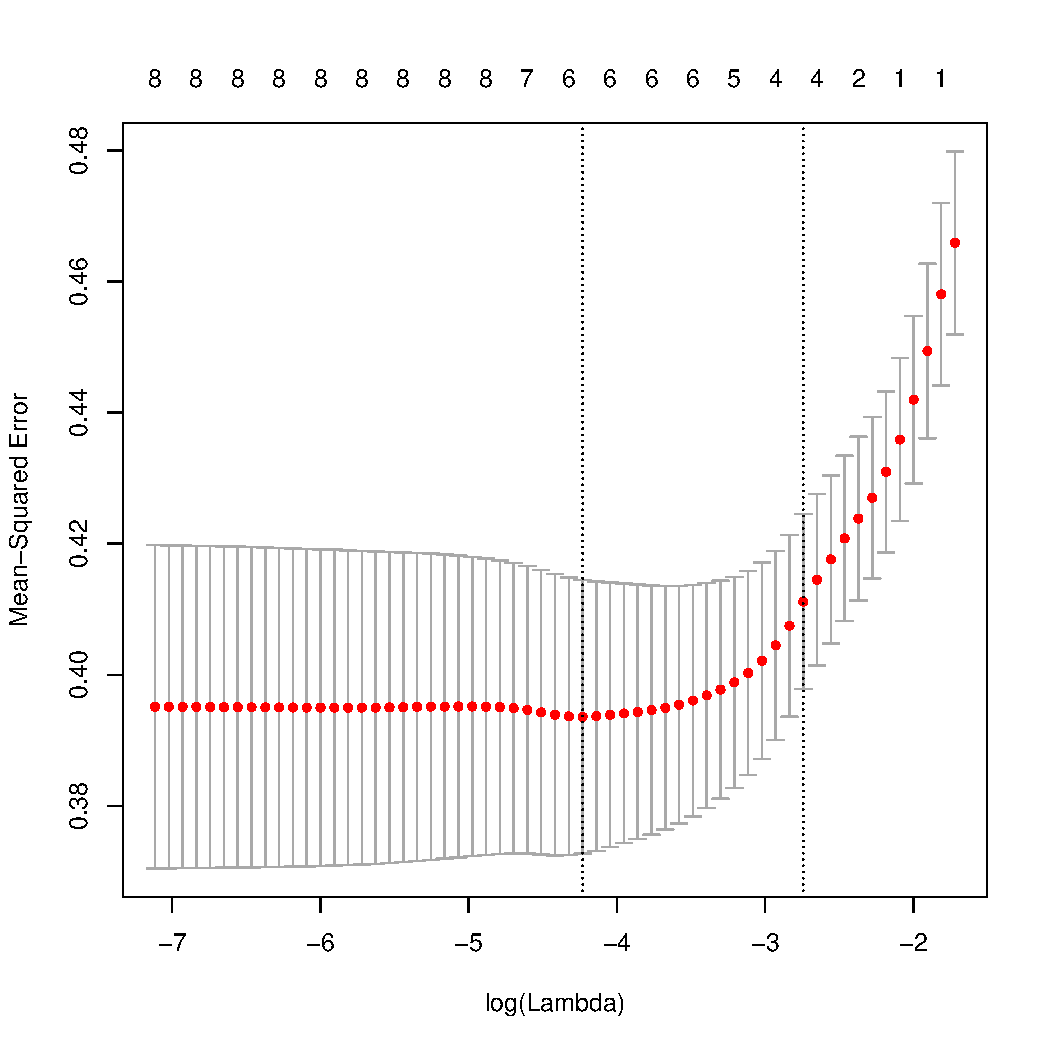
\includegraphics[width=\maxwidth]{figure/minimal-SouthAfrica1} 
\begin{kframe}\begin{alltt}
\hlstd{lasso_train} \hlkwb{<-} \hlkwd{predict}\hlstd{(lasso,} \hlkwd{as.matrix}\hlstd{(X_train),} \hlkwc{s} \hlstd{= cv.lasso}\hlopt{$}\hlstd{lambda.min,} \hlkwc{type} \hlstd{=} \hlstr{"class"}\hlstd{)}
\hlstd{Train.error[}\hlnum{4}\hlstd{, ]} \hlkwb{<-} \hlkwd{sum}\hlstd{(}\hlkwd{as.factor}\hlstd{(lasso_train)} \hlopt{!=} \hlkwd{as.factor}\hlstd{(Response_train))}\hlopt{/}\hlkwd{length}\hlstd{(Response_train)}
\hlkwd{sum}\hlstd{(}\hlkwd{as.factor}\hlstd{(lasso_train)} \hlopt{!=} \hlkwd{as.factor}\hlstd{(Response_train))}\hlopt{/}\hlkwd{length}\hlstd{(Response_train)}
\end{alltt}
\begin{verbatim}
## [1] 0.3033
\end{verbatim}
\begin{alltt}
\hlstd{lasso_test} \hlkwb{<-} \hlkwd{predict}\hlstd{(lasso,} \hlkwd{as.matrix}\hlstd{(X_test),} \hlkwc{s} \hlstd{= cv.lasso}\hlopt{$}\hlstd{lambda.min,} \hlkwc{type} \hlstd{=} \hlstr{"class"}\hlstd{)}
\hlstd{Test.error[}\hlnum{4}\hlstd{, ]} \hlkwb{<-} \hlkwd{sum}\hlstd{(}\hlkwd{as.factor}\hlstd{(lasso_test)} \hlopt{!=} \hlkwd{as.factor}\hlstd{(Response_test))}\hlopt{/}\hlkwd{length}\hlstd{(Response_test)}
\hlkwd{sum}\hlstd{(}\hlkwd{as.factor}\hlstd{(lasso_test)} \hlopt{!=} \hlkwd{as.factor}\hlstd{(Response_test))}\hlopt{/}\hlkwd{length}\hlstd{(Response_test)}
\end{alltt}
\begin{verbatim}
## [1] 0.2531
\end{verbatim}
\begin{alltt}
\hlcom{# Detect false positive and false negative}
\hlkwd{fpfn}\hlstd{(lasso_test, Response_test)}
\end{alltt}
\begin{verbatim}
## False Positive False Negative 
##              9             32
\end{verbatim}
\begin{alltt}
\hlkwd{row.names}\hlstd{(Train.error)} \hlkwb{<-} \hlkwd{c}\hlstd{(}\hlstr{"LDA"}\hlstd{,} \hlstr{"QDA"}\hlstd{,} \hlstr{"Logit"}\hlstd{,} \hlstr{"Logit with Lasso"}\hlstd{)}
\hlkwd{with}\hlstd{(}\hlkwd{plot}\hlstd{(Train.error,} \hlkwc{type} \hlstd{=} \hlstr{"b"}\hlstd{,} \hlkwc{main} \hlstd{=} \hlstr{"Training and Test Error"}\hlstd{,} \hlkwc{ylim} \hlstd{=} \hlkwd{c}\hlstd{(}\hlnum{0.2}\hlstd{,} \hlnum{0.33}\hlstd{)),}
    \hlkwd{text}\hlstd{(}\hlkwc{x} \hlstd{= Train.error,} \hlkwc{labels} \hlstd{=} \hlkwd{c}\hlstd{(}\hlstr{"LDA"}\hlstd{,} \hlstr{"QDA"}\hlstd{,} \hlstr{"Logit"}\hlstd{,} \hlstr{"Lasso"}\hlstd{),} \hlkwc{pos} \hlstd{=} \hlnum{3}\hlstd{))}
\hlkwd{lines}\hlstd{(Test.error,} \hlkwc{lty} \hlstd{=} \hlnum{2}\hlstd{)}
\hlkwd{legend}\hlstd{(}\hlstr{"bottomright"}\hlstd{,} \hlkwd{c}\hlstd{(}\hlstr{"Train Error"}\hlstd{,} \hlstr{"Test Error"}\hlstd{),} \hlkwc{lty} \hlstd{=} \hlkwd{c}\hlstd{(}\hlnum{1}\hlstd{,} \hlnum{2}\hlstd{))}
\end{alltt}
\end{kframe}
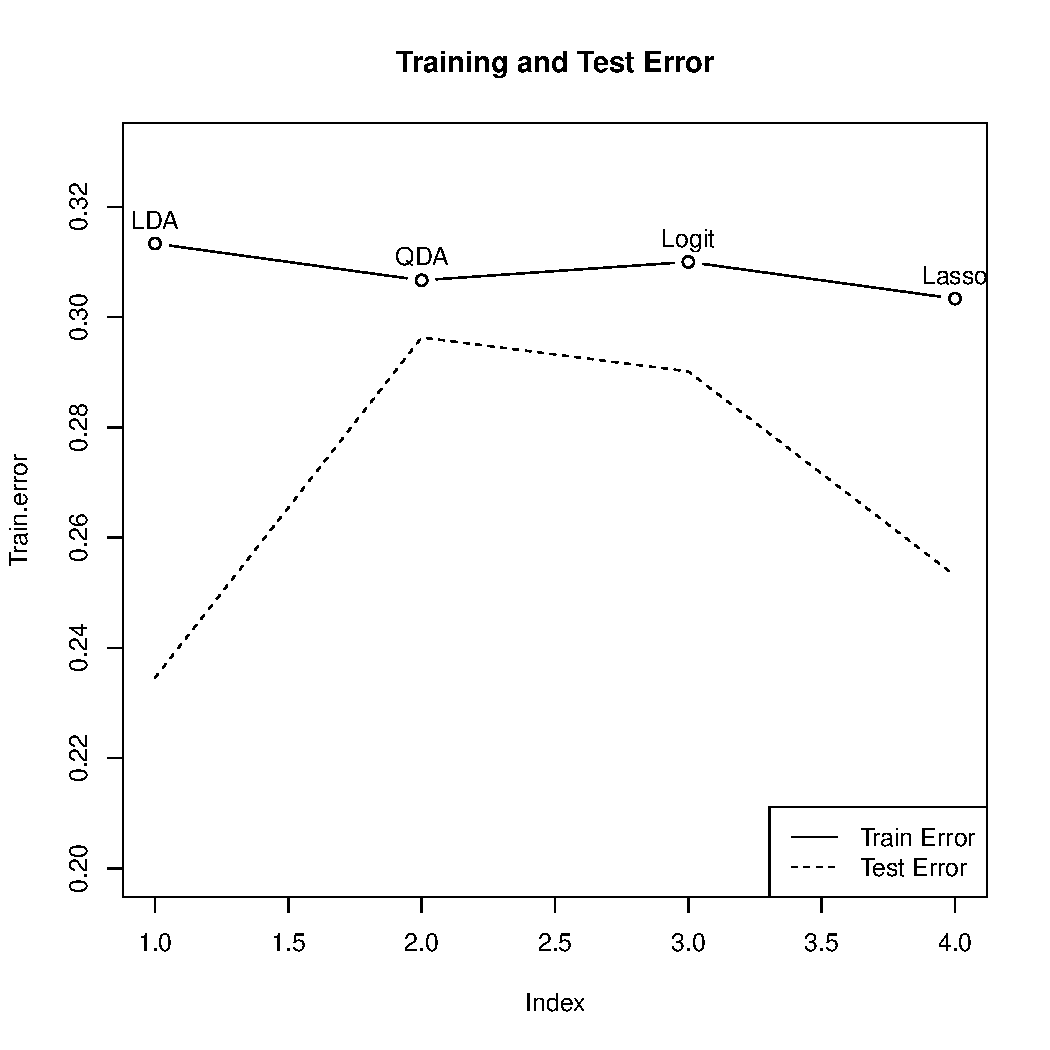
\includegraphics[width=\maxwidth]{figure/minimal-SouthAfrica2} 
\begin{kframe}\begin{alltt}
\hlstd{FPFN} \hlkwb{<-} \hlkwd{rbind}\hlstd{(}\hlkwd{fpfn}\hlstd{(LDA_test, Response_test),} \hlkwd{fpfn}\hlstd{(QDA_test, Response_test),} \hlkwd{fpfn}\hlstd{(logistic_test,}
    \hlstd{Response_test),} \hlkwd{fpfn}\hlstd{(lasso_test, Response_test))}
\hlkwd{row.names}\hlstd{(FPFN)} \hlkwb{<-} \hlkwd{c}\hlstd{(}\hlstr{"LDA"}\hlstd{,} \hlstr{"QDA"}\hlstd{,} \hlstr{"Logit"}\hlstd{,} \hlstr{"Logit with Lasso"}\hlstd{)}
\hlkwd{with}\hlstd{(}\hlkwd{plot}\hlstd{(FPFN,} \hlkwc{main} \hlstd{=} \hlstr{"False Positive & False Negative"}\hlstd{,} \hlkwc{ylim} \hlstd{=} \hlkwd{c}\hlstd{(}\hlnum{15}\hlstd{,} \hlnum{40}\hlstd{),} \hlkwc{xlim} \hlstd{=} \hlkwd{c}\hlstd{(}\hlnum{5}\hlstd{,} \hlnum{35}\hlstd{)),}
    \hlkwd{text}\hlstd{(}\hlkwc{x} \hlstd{= FPFN[,} \hlnum{1}\hlstd{],} \hlkwc{y} \hlstd{= FPFN[,} \hlnum{2}\hlstd{],} \hlkwc{labels} \hlstd{=} \hlkwd{c}\hlstd{(}\hlstr{"LDA"}\hlstd{,} \hlstr{"QDA"}\hlstd{,} \hlstr{"Logit"}\hlstd{,} \hlstr{"Logit with Lasso"}\hlstd{),}
        \hlkwc{pos} \hlstd{=} \hlnum{3}\hlstd{))}
\end{alltt}
\end{kframe}
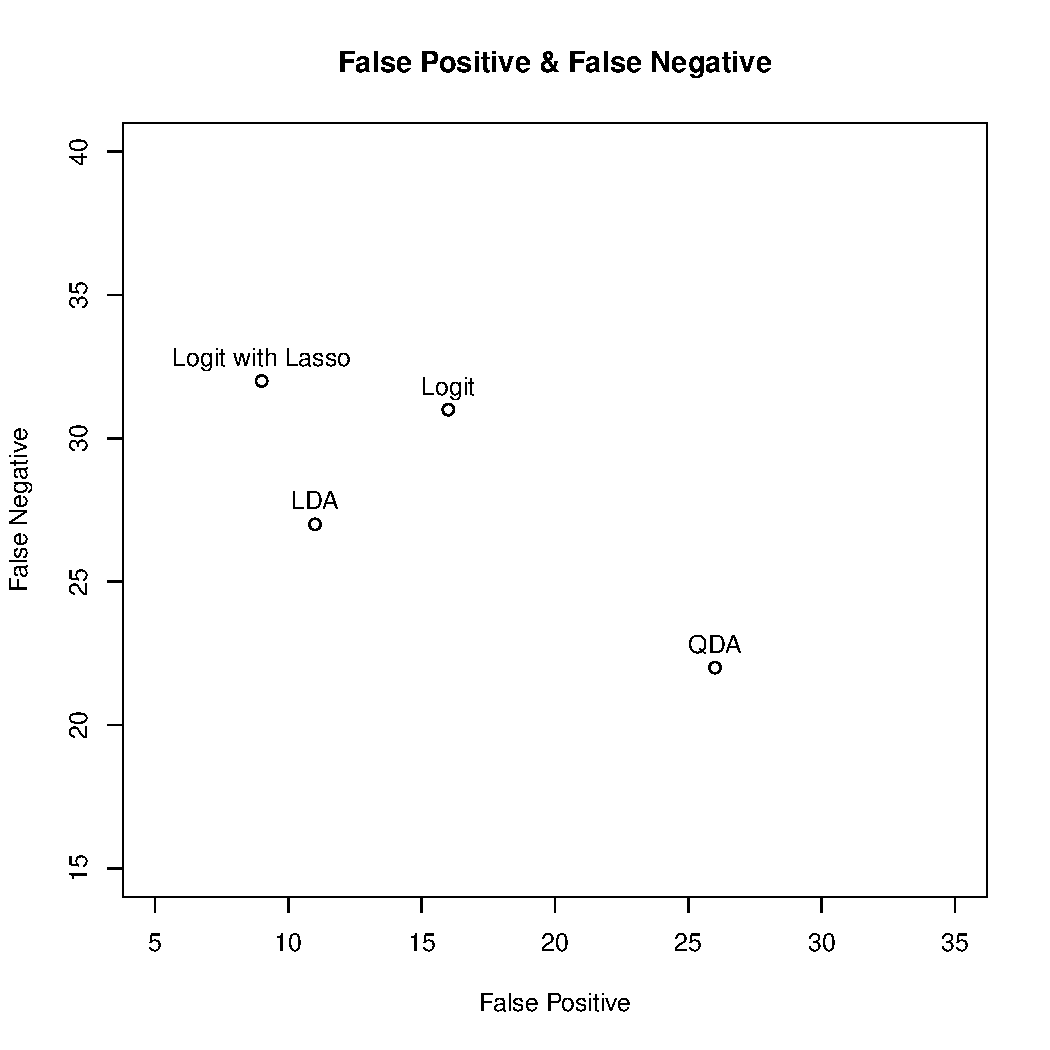
\includegraphics[width=\maxwidth]{figure/minimal-SouthAfrica3} 

\end{knitrout}


\end{document}
